% !TeX root = ../thesis.tex
\section{Bitcoin: platba, blok a dátový graf}
\label{sec:bitcoin}

Bitcoin je decentralizovaný platobný systém, ktorý umožňuje prevod
digitálnej hodnoty bez centrálneho správcu. \textcite{nakamoto2008bitcoin}
v pôvodnom návrhu z roku 2008 opísal spôsob, ako môže sieť účastníkov
overovať platby a vytvárať spoločnú históriu transakcií. Menovou
jednotkou systému je bitcoin, označovaný skratkou BTC. Jeho emisiu
určujú pravidlá protokolu, ktoré obmedzujú celkové množstvo na približne
21 miliónov BTC~\cite{bitcoinFaq}.

Pre túto prácu je podstatná verejná dostupnosť transakčných záznamov
a ich vzájomné prepojenie. Umožňujú rekonštruovať vzťahy medzi
transakciami a odvodiť z nich údaje využiteľné pri analýze blockchainu.
Význam týchto údajov však závisí od spôsobu, akým transakcie vznikajú,
overujú sa a zaraďujú do blokov.

\tikzset{
  btcbox/.style={draw=black!65,rounded corners=2pt,
    line width=0.6pt,align=center,font=\small,inner sep=5pt},
  btcarrow/.style={-{Latex[length=2mm]},draw=black!75,line width=0.7pt},
  btcnote/.style={font=\footnotesize,align=center}
}

\subsection{Bitcoinová sieť a blockchain}

Bitcoinová sieť má usporiadanie typu peer-to-peer: jednotlivé uzly
komunikujú priamo so svojimi susedmi a odovzdávajú si transakcie
a bloky. Transakcia predstavuje záznam o prevode hodnoty podľa
pravidiel protokolu. Blok združuje transakcie do spoločného záznamu
a obsahuje hlavičku s údajmi potrebnými na jeho overenie. Úplný uzol
samostatne kontroluje platnosť prijatých údajov; rozhodnutie
nepreberá od banky ani od prevádzkovateľa iného uzla. Dokumentácia
Bitcoin Developer Guide opisuje túto komunikáciu ako základ
distribuovaného overovania~\cite{bitcoinDevP2P}.

Bloky sú prepojené do reťazca označovaného ako \emph{blockchain}.
Hlavička každého bloku okrem počiatočného obsahuje kryptografický
odtlačok hlavičky predchádzajúceho bloku. Kryptografický odtlačok,
ďalej \emph{hash}, je hodnota pevnej dĺžky vypočítaná zo vstupných
údajov. Zmena týchto údajov sa s veľmi vysokou pravdepodobnosťou
prejaví zmenou hashu. Odkaz na predchádzajúci blok tak viaže nový
blok na konkrétnu podobu predchádzajúcej histórie.
Obrázok~\ref{fig:block-transaction-io} odlišuje smer týchto odkazov
od smeru rastu reťazca.

\begin{figure}[htbp]
  \centering
  \begin{tikzpicture}
    \node[btcbox,fill=blue!6,text width=34mm,minimum height=20mm]
      (b0) at (0,0) {\textbf{Blok $h-1$}\\Odkaz na rodiča\\Transakcie};
    \node[btcbox,fill=blue!6,text width=34mm,minimum height=20mm]
      (b1) at (4.8,0) {\textbf{Blok $h$}\\Odkaz na blok $h-1$\\Transakcie};
    \node[btcbox,fill=blue!6,text width=34mm,minimum height=20mm]
      (b2) at (9.6,0) {\textbf{Blok $h+1$}\\Odkaz na blok $h$\\Transakcie};
    \draw[btcarrow] (b1.west) -- node[above,btcnote]{hash} (b0.east);
    \draw[btcarrow] (b2.west) -- node[above,btcnote]{hash} (b1.east);
    \draw[btcarrow] (-1.5,-1.75) -- node[above,btcnote]
      {poradie blokov a smer rastu reťazca} (11.1,-1.75);
  \end{tikzpicture}
  \caption[Prepojenie blokov pomocou hashov hlavičiek]{Prepojenie blokov pomocou hashov ich hlavičiek.
  Odkazy smerujú k predchádzajúcim blokom; reťazec rastie opačným
  smerom. Vlastné spracovanie podľa~\cite{bitcoinDevBlockChain}.}
  \label{fig:block-transaction-io}
\end{figure}

Poradie bloku v reťazci vyjadruje jeho \emph{výška}, pričom počiatočný
blok má výšku nula. Pri dočasnom rozvetvení môžu existovať viaceré bloky na rovnakej
výške. Konkrétny blok sa preto identifikuje hashom jeho hlavičky.
Hlavička obsahuje aj koreň Merkleovho stromu, ktorý sa postupným
hashovaním dvojíc identifikátorov transakcií vypočíta pre transakcie
daného bloku. Zmena týchto identifikátorov sa premietne do hlavičky
a naruší nadväzujúce hashové odkazy~\cite{bitcoinDevBlockReference}.
Odolnosť histórie voči prepisovaniu navyše závisí od dôkazu práce,
ktorý je opísaný v podkapitole~\ref{sec:bitcoin-mining}.

\subsection{Štruktúra transakcie a model UTXO}
\label{sec:bitcoin-utxo}

Bežná bitcoinová transakcia\footnote{Výnimkou je \emph{coinbase},
prvá transakcia bloku, ktorá nemíňa staršie výstupy a umožňuje
ťažiarovi uplatniť nárok na blokovú subvenciu a poplatky~\cite{bitcoinDevMining}.}
spotrebúva existujúce výstupy a vytvára nové. Každý výstup obsahuje
hodnotu v satoshi a skript určujúci podmienky jej minutia;
jeden BTC zodpovedá $100\,000\,000$ satoshi. Výstup, ktorý zatiaľ
neminula iná transakcia, sa označuje ako \emph{UTXO}
(angl. \emph{unspent transaction output}).

Vstup nasledujúcej transakcie odkazuje na míňaný výstup
identifikátorom pôvodnej transakcie \texttt{txid} a poradovým
indexom \texttt{vout}. Výstup sa spotrebuje celý; prípadný zvyšok
sa vracia prostredníctvom nového výstupu (\emph{change}), ako
znázorňuje obrázok~\ref{fig:utxo-example}. Poplatok predstavuje
rozdiel medzi súčtom hodnôt míňaných výstupov a súčtom hodnôt
nových výstupov~\cite{bitcoinDevTransactions}.

\begin{figure}[htbp]
  \centering
  \begin{tikzpicture}
    \node[btcnote] at (-4.7,2) {Existujúce UTXO};
    \node[btcnote] at (4.7,2) {Nové výstupy};
    \node[btcbox,fill=blue!6,text width=34mm,minimum height=15mm]
      (a) at (-4.7,1) {Výstup $(\texttt{txid}_A,0)$\\0,6 BTC};
    \node[btcbox,fill=blue!6,text width=34mm,minimum height=15mm]
      (b) at (-4.7,-1) {Výstup $(\texttt{txid}_B,0)$\\0,4 BTC};
    \node[btcbox,fill=black!4,text width=27mm,minimum height=18mm]
      (t) at (0,0) {Transakcia $T$\\2 vstupy\\2 výstupy};
    \node[btcbox,fill=blue!6,text width=34mm,minimum height=15mm]
      (o0) at (4.7,1) {Výstup 0: 0,8 BTC\\platba príjemcovi};
    \node[btcbox,fill=blue!6,text width=34mm,minimum height=15mm]
      (o1) at (4.7,-1) {Výstup 1: 0,19 BTC\\vrátený zvyšok};
    \draw[btcarrow] (a.east) -- (t.north west);
    \draw[btcarrow] (b.east) -- (t.south west);
    \draw[btcarrow] (t.north east) -- (o0.west);
    \draw[btcarrow] (t.south east) -- (o1.west);
    \node[btcnote] at (0,-2.25)
      {Poplatok: $1-(0{,}8+0{,}19)=0{,}01$ BTC};
  \end{tikzpicture}
  \caption[Spotrebovanie UTXO a vytvorenie nových výstupov]{Spotrebovanie dvoch UTXO a vytvorenie dvoch nových výstupov.~\cite{bitcoinDevTransactions}.}
  \label{fig:utxo-example}
\end{figure}

\subsection{Autorizácia transakcií a správa kľúčov}

Na platné minutie UTXO nestačí poznať jeho identifikátor.
Vstup musí splniť podmienky skriptu príslušného výstupu.
V bežných prípadoch ide o overenie digitálneho podpisu.
\emph{Súkromný kľúč} je tajná hodnota používaná pri podpisovaní;
zodpovedajúci \emph{verejný kľúč} umožňuje podpis overiť bez
sprístupnenia súkromného kľúča. Existujú aj podmienky vyžadujúce viac
podpisov alebo uplynutie určitého času. Platný podpis je teda
súčasťou autorizácie, nie náhradou kontroly ostatných pravidiel
transakcie~\cite{bitcoinDevTransactions}.

Bitcoinová \emph{adresa} je používateľsky čitateľný, kódovaný zápis
údajov, z ktorých možno pre podporovaný typ výstupu zostaviť jeho
podmienku minutia. Presný význam závisí od typu adresy:
môže súvisieť s verejným kľúčom alebo so skriptom.
Adresu preto nemožno všeobecne stotožniť s verejným kľúčom.
V samotnej transakcii sa ukladá výstupný skript; adresa je jeho
bežne používanou reprezentáciou pre príslušný typ výstupu.

\emph{Peňaženka} spravuje kľúče, sleduje dostupné výstupy a zostavuje
transakcie. Jedna peňaženka môže používať mnoho adries, napríklad
odlišnú adresu na každé prijatie platby a ďalšiu na vrátenie zvyšku.
Hodnota, s ktorou môže používateľ disponovať, vyplýva z výstupov,
ktorých podmienky dokáže splniť. Dokumentácia peňaženiek preto
oddeľuje správu kľúčov od záznamov transakcií uložených
v blockchaine~\cite{bitcoinDevWallets}.

\subsection{Šírenie transakcií, ťažba a potvrdenia}
\label{sec:bitcoin-mining}

Po zostavení a autorizácii môže peňaženka odoslať transakciu do siete.
Uzol ju overí a podľa lokálnych pravidiel môže zaradiť do
\emph{mempoolu}, množiny nepotvrdených transakcií, a ďalej šíriť.
Každý uzol spravuje vlastný mempool; prijatie transakcie do tejto
množiny nezaručuje jej potvrdenie.

Ťažiar vyberie transakcie do kandidátskeho bloku a hľadá hlavičku,
ktorej hash neprevyšuje cieľ určený náročnosťou. Tento mechanizmus
sa nazýva \emph{dôkaz práce} (angl. \emph{proof of work}, PoW).
Úplné uzly následne overia blok aj jeho transakcie, ako znázorňuje
obrázok~\ref{fig:transaction-lifecycle}. Úprava náročnosti smeruje
k priemernému intervalu približne desať minút medzi blokmi,
nie k pevnej lehote potvrdenia transakcie~\cite{bitcoinDevMining}.

\begin{figure}[htbp]
  \centering
  \begin{tikzpicture}
    \node[btcbox,fill=blue!6,text width=33mm,minimum height=18mm]
      (w) at (0,0) {Peňaženka\\zostavenie a podpis\\transakcie};
    \node[btcbox,fill=blue!6,text width=33mm,minimum height=18mm]
      (n) at (4.8,0) {Úplný uzol\\kontrola transakcie\\lokálny mempool};
    \node[btcbox,fill=blue!6,text width=33mm,minimum height=18mm]
      (m) at (9.6,0) {Ťažiar\\kandidátsky blok\\a dôkaz práce};
    \node[btcbox,fill=black!4,text width=33mm,minimum height=18mm]
      (b) at (9.6,-2.5) {Nový blok\\šírenie do siete};
    \node[btcbox,fill=black!4,text width=33mm,minimum height=18mm]
      (v) at (4.8,-2.5) {Úplné uzly\\overenie bloku\\a jeho transakcií};
    \node[btcbox,fill=blue!6,text width=33mm,minimum height=18mm]
      (c) at (0,-2.5) {Aktívny reťazec\\prvé potvrdenie\\transakcie};
    \draw[btcarrow] (w.east) -- (n.west);
    \draw[btcarrow] (n.east) -- (m.west);
    \draw[btcarrow] (m.south) -- (b.north);
    \draw[btcarrow] (b.west) -- (v.east);
    \draw[btcarrow] (v.west) -- (c.east);
  \end{tikzpicture}
  \caption[Zaradenie transakcie do aktívneho reťazca]{Priebeh úspešného zaradenia transakcie do aktívneho reťazca.
  Schéma nevyjadruje záruku prijatia ani pevné časové intervaly.
  Vlastné spracovanie podľa~\cite{bitcoinDevP2P,bitcoinDevMining}.}
  \label{fig:transaction-lifecycle}
\end{figure}

Spomedzi platných vetiev uzly vyberajú reťazec s najväčšou
kumulatívnou prácou. Spoločné pravidlá overovania a výberu reťazca
tvoria základ \emph{konsenzu}. Transakcia získava prvé
\emph{potvrdenie} zaradením do aktívneho reťazca a každým
nadväzujúcim blokom ďalšie. Pri zmene aktívnej vetvy, nazývanej
\emph{reorganizácia}, môže potvrdenie stratiť
(obrázok~\ref{fig:bitcoin-confirmations}). Viac potvrdení sťažuje
nahradenie histórie, neposkytuje však absolútnu záruku
nezvratnosti~\cite{nakamoto2008bitcoin,bitcoinDevBlockChain}.

\begin{figure}[htbp]
  \centering
  \begin{tikzpicture}
    \node[btcbox,fill=black!4,text width=30mm,minimum height=16mm]
      (common) at (0,0) {Blok $h$\\spoločný predchodca};
    \node[btcbox,fill=blue!6,text width=33mm,minimum height=16mm]
      (a1) at (4.8,1.2) {Blok $h+1$\\vetva A, transakcia $T$};
    \node[btcbox,fill=blue!6,text width=33mm,minimum height=16mm]
      (a2) at (9.6,1.2) {Blok $h+2$\\$T$: 2 potvrdenia};
    \node[btcbox,fill=black!4,text width=33mm,minimum height=16mm]
      (b1) at (4.8,-1.2) {Blok $h+1$\\vetva B};
    \draw[btcarrow] (a1.west) -- (common.north east);
    \draw[btcarrow] (a2.west) -- (a1.east);
    \draw[btcarrow] (b1.west) -- (common.south east);
    \node[btcnote] at (9.6,2.3) {aktívna vetva A};
    \node[btcnote,text width=40mm] at (9.6,-1.2)
      {platný blok vetvy B\\mimo aktívneho reťazca};
  \end{tikzpicture}
  \caption[Dočasné rozvetvenie blockchainu a potvrdenia]{Dočasné rozvetvenie blockchainu. V príklade majú bloky
  rovnakú prácu, preto vetva A predstavuje väčšiu kumulatívnu prácu
  než vetva B. Šípky označujú odkazy na predchádzajúce bloky.
  Vlastné spracovanie podľa~\cite{bitcoinDevBlockChain}.}
  \label{fig:bitcoin-confirmations}
\end{figure}

\subsection{Veľkosť transakcií a poplatky}

Pre výpočet poplatku $f$ bežnej transakcie platí
\begin{equation}
  f=\sum_{i=1}^{n}v_i^{\mathrm{in}}
    -\sum_{j=1}^{m}v_j^{\mathrm{out}},
  \label{eq:bitcoin-fee}
\end{equation}
kde $v_i^{\mathrm{in}}$ označujú hodnoty míňaných výstupov
a $v_j^{\mathrm{out}}$ hodnoty nových výstupov.

Obmedzená kapacita bloku ovplyvňuje výber transakcií aj ich poplatky.
Pri mechanizme \emph{SegWit} (angl. \emph{Segregated Witness}) sa
údaje svedkov potrebné na overenie minutia oddeľujú od základnej
serializácie, z ktorej sa počíta \texttt{txid}. BIP~141~\cite{bip141}
rozlišuje veľkosť v bajtoch, váhu $W$ a virtuálnu veľkosť $V$:
\begin{equation}
  W=3B_{\mathrm{base}}+B_{\mathrm{total}},
  \qquad
  V=\left\lceil\frac{W}{4}\right\rceil,
  \label{eq:bitcoin-weight}
\end{equation}
kde $B_{\mathrm{base}}$ je veľkosť serializácie bez údajov svedkov
a $B_{\mathrm{total}}$ veľkosť vrátane nich. Váha sa udáva vo váhových
jednotkách (WU), virtuálna veľkosť vo virtuálnych bajtoch (vB).
Limit váhy bloku je $4\,000\,000$ WU.

Poplatok $f$ z rovnice~\eqref{eq:bitcoin-fee} treba odlišovať od
poplatkovej sadzby $r=f/V$, vyjadrenej v satoshi na virtuálny bajt
(sat/vB). Ťažiari môžu uprednostňovať transakcie s vyššou sadzbou,
pričom rešpektujú závislosti od nepotvrdených predchodcov.

\subsection{Grafová reprezentácia transakcií}
\label{sec:bitcoin-graph}

Odkazy vstupov na staršie výstupy umožňujú zostaviť smerovaný graf
$G=(V,E)$. V transakčnom grafe každý vrchol $T_i\in V$ predstavuje
jednu transakciu. Hrana $(T_i,T_j)\in E$ existuje vtedy, keď
transakcia $T_j$ míňa aspoň jeden výstup transakcie $T_i$.
Jej smer vyjadruje závislosť minutia, od vytvorenia výstupu
k jeho spotrebovaniu. Takto vytvorený graf platných transakcií
je acyklický: transakcia nemôže priamo ani nepriamo minúť
svoj vlastný budúci výstup.

\begin{figure}[htbp]
  \centering
  \begin{tikzpicture}
    \node[btcbox,fill=blue!6,text width=23mm,minimum height=12mm]
      (a) at (0,1.2) {Transakcia $A$};
    \node[btcbox,fill=blue!6,text width=23mm,minimum height=12mm]
      (b) at (0,-1.2) {Transakcia $B$};
    \node[btcbox,fill=black!4,text width=23mm,minimum height=14mm]
      (t) at (4.8,0) {Transakcia $T$};
    \node[btcbox,fill=blue!6,text width=23mm,minimum height=12mm]
      (d) at (9.6,1.2) {Transakcia $D$};
    \node[btcbox,fill=blue!6,text width=23mm,minimum height=12mm]
      (e) at (9.6,-1.2) {Transakcia $E$};
    \draw[btcarrow] (a.east) -- node[above,btcnote]
      {výstup 0} (t.north west);
    \draw[btcarrow] (b.east) -- node[below,btcnote]
      {výstup 0} (t.south west);
    \draw[btcarrow] (t.north east) -- node[above,btcnote]
      {výstup 0} (d.west);
    \draw[btcarrow] (t.south east) -- node[below,btcnote]
      {výstup 1} (e.west);
  \end{tikzpicture}
  \caption[Grafová reprezentácia transakčných väzieb]{Transakčný graf nadväzujúci na príklad UTXO.
  Transakcia $T$ míňa výstupy transakcií $A$ a $B$; jej nové výstupy
  neskôr míňajú transakcie $D$ a $E$. Každá šípka smeruje
  od rodičovskej transakcie k potomkovi.}
  \label{fig:bitcoin-transaction-graph}
\end{figure}

Obrázok~\ref{fig:bitcoin-transaction-graph} ukazuje prechod od výstupov
z obrázka~\ref{fig:utxo-example} k vrcholom grafu.
Ak jedna transakcia míňa viac výstupov toho istého predchodcu,
jednoduchý graf ich zlúči do jednej hrany. Detailnejšia reprezentácia
môže zachovať jednotlivé odkazy aj ich hodnoty. Voľba reprezentácie
tak ovplyvňuje napríklad počet hrán a interpretáciu stupňa vrcholu.
Rodičovská a potomkovská transakcia pritom môžu byť súčasťou
toho istého bloku; závislosť nevyžaduje rozdielnu výšku blokov.

Transakčný graf sa odlišuje od grafu adries, v ktorom vrcholy
predstavujú adresy. Pri viacerých vstupoch a výstupoch protokol
neurčuje, ktorá časť konkrétneho vstupu financuje konkrétny výstup.
Prevod transakcie na vážené hrany medzi adresami preto vyžaduje
zvolené pravidlo priradenia hodnoty.

\subsection{Pranie špinavých peňazí a miešanie transakcií}
\label{sec:bitcoin-laundering}

Pri praní špinavých peňazí páchatelia zakrývajú nezákonný pôvod
výnosov a ich väzbu na trestnú činnosť. V prostredí Bitcoinu môžu
prevádzať už získané bitcoiny alebo doň vnášať výnosy pôvodne
získané v inej forme. Europol~\cite{europol2022crypto} opisuje
využívanie sprostredkovateľských služieb aj profesionálnych sietí,
ktoré pre iných páchateľov zabezpečujú presuny a výmenu takýchto
prostriedkov. Pre grafovú analýzu je podstatné, ako tieto postupy
menia pozorovateľné transakčné väzby.

Páchatelia môžu rozdeľovať prostriedky medzi viacero adries,
spájať ich do spoločných transakcií a presúvať cez viaceré služby.
Organizácia FATF (angl. \emph{Financial Action Task Force}) medzi
rizikové vzorce zaraďuje rýchle nadväzujúce prevody či zhromažďovanie
platieb z viacerých zdrojov bez zrejmého ekonomického
dôvodu~\cite{fatf2020redflags}.

Jedným z pozorovateľných vzorcov je \emph{peeling chain}, teda
reťazec transakcií, v ktorom sa postupne oddeľujú platby a vracaný
zvyšok sa používa v ďalšej transakcii. Kappos
a spoluautori~\cite{kappos2022peel} využívajú tieto väzby na
sledovanie prostriedkov a overovanie zoskupenia adries.
Obrázok~\ref{fig:bitcoin-peeling-chain} dopĺňa tento vzorec
o následné spojenie oddelených častí v transakcii $K$, ktorá
vytvorí výstup pre spoločnú adresu $a$. V modelovom scenári
páchateľ ovláda zobrazené prevody a ďalšími transakciami sa pokúša
sťažiť sledovanie nelegálnych výnosov. Odkazy medzi míňanými
výstupmi pritom zostávajú verejné.

\begin{center}
  \begin{minipage}{\textwidth}
  \centering
  \captionsetup{type=figure}
  \begin{tikzpicture}
    \node[btcnote,text width=120mm] at (4.8,1.2)
      {Modelový scenár: rozdelenie a opätovné spojenie nelegálnych výnosov};
    \node[btcbox,font=\normalsize,fill=blue!6,text width=28mm,minimum height=14mm]
      (t1) at (0,0) {Transakcia $T_1$};
    \node[btcbox,font=\normalsize,fill=blue!6,text width=28mm,minimum height=14mm]
      (t2) at (4.8,0) {Transakcia $T_2$};
    \node[btcbox,font=\normalsize,fill=blue!6,text width=28mm,minimum height=14mm]
      (t3) at (9.6,0) {Transakcia $T_3$};
    \node[btcbox,font=\normalsize,fill=black!4,text width=28mm,minimum height=14mm]
      (p1) at (0,-2.2) {Transakcia $P_1$};
    \node[btcbox,font=\normalsize,fill=black!4,text width=28mm,minimum height=14mm]
      (p2) at (4.8,-2.2) {Transakcia $P_2$};
    \node[btcbox,font=\normalsize,fill=black!4,text width=28mm,minimum height=14mm]
      (p3) at (9.6,-2.2) {Transakcia $P_3$};
    \node[btcbox,font=\normalsize,fill=orange!10,text width=49mm,minimum height=22mm]
      (k) at (4.8,-5) {Transakcia $K$\\3 vstupy, 1 výstup\\výstup pre spoločnú adresu $a$};
    \draw[btcarrow] (t1.east) -- node[above,btcnote]{zvyšok} (t2.west);
    \draw[btcarrow] (t2.east) -- node[above,btcnote]{zvyšok} (t3.west);
    \draw[btcarrow] (t1.south) -- node[right,btcnote]{platba} (p1.north);
    \draw[btcarrow] (t2.south) -- node[right,btcnote]{platba} (p2.north);
    \draw[btcarrow] (t3.south) -- node[right,btcnote]{platba} (p3.north);
    \draw[btcarrow] (p1.south) -- (k.north west);
    \draw[btcarrow] (p2.south) -- (k.north);
    \draw[btcarrow] (p3.south) -- (k.north east);
  \end{tikzpicture}
  \caption[Peeling chain a následné spojenie oddelených výstupov]{Modelový scenár pokusu o zakrytie pôvodu prostriedkov.
  Transakcie $P_i$ míňajú oddelené výstupy transakcií $T_i$;
  transakcia $K$ následne spotrebuje ich výstupy a vytvorí jeden
  výstup pre adresu $a$. Všetky šípky označujú závislosti minutia.
  \emph{peeling chain} podľa~\cite{kappos2022peel}.}
  \label{fig:bitcoin-peeling-chain}
  \end{minipage}
\end{center}

\emph{Miešacie služby}, označované aj ako \emph{mixéry} alebo
\emph{tumblery}, sťažujú priradenie vkladu ku konkrétnej následnej
výplate. Pri mixéri s úschovou používateľ prevedie prostriedky
pod kontrolu prevádzkovateľa, ktorý zabezpečí výplatu na určené
adresy z prostriedkov služby. Ruffing
a spoluautori~\cite{ruffing2014coinshuffle} upozorňujú, že takýto
model vyžaduje dôveru v prevádzkovateľa: ten môže poznať väzby
medzi vkladmi a výplatami alebo si prostriedky ponechať.
Transakčné záznamy pritom zostávajú v blockchaine.

Konkrétnym prípadom zneužitia mixéra bola služba Helix.
Ministerstvo spravodlivosti USA~\cite{doj2026helix} uvádza,
že v rokoch 2014 až 2017 spracovala približne $354\,000$ BTC,
pričom značná časť prostriedkov smerovala z nelegálnych trhovísk
alebo na ne. Jej prevádzkovateľ sa v roku 2021 priznal k účasti
na praní špinavých peňazí.

Od tohto modelu sa odlišuje \emph{CoinJoin}, pri ktorom viacerí
účastníci zostavia jednu transakciu s vlastnými vstupmi a dohodnutými
výstupmi.

\begin{center}
  \begin{minipage}{\textwidth}
  \centering
  \captionsetup{type=figure}
  \begin{tikzpicture}
    \node[btcnote] at (0,2.65) {Míňané UTXO};
    \node[btcnote] at (9.6,2.65) {Nové výstupy};
    \node[btcbox,fill=blue!6,text width=29mm,minimum height=13mm]
      (ia) at (0,1.5) {Účastník $A$\\0,101 BTC};
    \node[btcbox,fill=blue!6,text width=29mm,minimum height=13mm]
      (ib) at (0,0) {Účastník $B$\\0,101 BTC};
    \node[btcbox,fill=blue!6,text width=29mm,minimum height=13mm]
      (ic) at (0,-1.5) {Účastník $C$\\0,101 BTC};
    \node[btcbox,fill=black!4,text width=33mm,minimum height=23mm]
      (cj) at (4.8,0) {Spoločná transakcia\\CoinJoin\\3 vstupy, 3 výstupy};
    \node[btcbox,fill=blue!6,text width=29mm,minimum height=13mm]
      (ox) at (9.6,1.5) {Výstup $X$\\0,100 BTC};
    \node[btcbox,fill=blue!6,text width=29mm,minimum height=13mm]
      (oy) at (9.6,0) {Výstup $Y$\\0,100 BTC};
    \node[btcbox,fill=blue!6,text width=29mm,minimum height=13mm]
      (oz) at (9.6,-1.5) {Výstup $Z$\\0,100 BTC};
    \draw[btcarrow] (ia.east) -- (cj.north west);
    \draw[btcarrow] (ib.east) -- (cj.west);
    \draw[btcarrow] (ic.east) -- (cj.south west);
    \draw[btcarrow] (cj.north east) -- (ox.west);
    \draw[btcarrow] (cj.east) -- (oy.west);
    \draw[btcarrow] (cj.south east) -- (oz.west);
    \node[btcnote,text width=110mm] at (4.8,-3.1)
      {Poplatok: $0{,}303-0{,}300=0{,}003$ BTC.};
  \end{tikzpicture}
  \caption[Spoločná transakcia typu CoinJoin]{Zjednodušený príklad CoinJoin s tromi účastníkmi.
  Šípky znázorňujú spotrebovanie UTXO a vznik výstupov, nie
  jednoznačné platby $A\to X$, $B\to Y$, $C\to Z$.
  ~\cite{ruffing2014coinshuffle,stutz2022coinjoin}.}
  \label{fig:bitcoin-coinjoin}
  \end{minipage}
\end{center}

Ďalším mechanizmom ochrany súkromia je \emph{CoinSwap}, pri ktorom
si účastníci vymieňajú kontrolu nad bitcoinovými výstupmi pomocou
vzájomne podmienených transakcií.
Vývojová dokumentácia projektu Teleport
Transactions~\cite{teleportCoinSwap} opisuje princíp takejto výmeny
v rámci Bitcoinu. Ide o odlišný mechanizmus od spoločnej
transakcie CoinJoin.

Používanie týchto nástrojov neposkytuje záruku anonymity.
Stütz a spoluautori~\cite{stutz2022coinjoin} ukázali, že analýza
transakcií pred miešaním a po ňom môže zúžiť množinu možných
priradení. CoinJoin zároveň slúži aj na ochranu finančného súkromia.
FATF preto zdôrazňuje potrebu hodnotiť rizikové indikátory v kontexte.~\cite{fatf2020redflags}.

\subsection{Podvody a ďalšie zdroje nelegálnych výnosov}
\label{sec:bitcoin-fraud}

Podvodné konanie sa často odohráva mimo blockchainu, hoci jeho
finančné dôsledky možno sledovať v transakčnom grafe. Pri falošných
investičných platformách páchatelia presviedčajú obete, aby vložili
bitcoiny, a v používateľskom rozhraní zobrazujú neexistujúce
výnosy. FBI~\cite{fbiCryptoInvestmentFraud} opisuje aj počiatočné
povolenie menších výberov na získanie dôvery a neskoršie požiadavky
na ďalšie platby pod zámienkou uvoľnenia prostriedkov.

Osobitným prípadom investičného podvodu je \emph{Ponziho schéma}.
Organizátori vyplácajú skorších účastníkov z vkladov nových
účastníkov namiesto výnosov zo skutočnej investičnej činnosti.
Časť obetí tak môže prijímať platby z tej istej schémy, do ktorej
predtým vložila prostriedky. Bartoletti
a spoluautori~\cite{bartoletti2018ponzi} skúmali takéto schémy
v bitcoinovom blockchaine a využili charakteristiky ich transakcií
na klasifikáciu súvisiacich adries.

Pri \emph{phishingu} páchatelia napodobňujú dôveryhodnú službu,
aby získali prístupové údaje alebo podnietili obeť k platbe.
Falošná technická podpora môže požadovať súkromný kľúč alebo
obnovovaciu frázu, z ktorej peňaženka odvodzuje kľúče.
Útočník so získanými kľúčmi môže vytvoriť platný podpis a previesť
dostupné prostriedky.~\cite{bitcoinScams,bitcoinDevTransactions}.

Ďalším zdrojom nelegálnych výnosov je \emph{ransomvér}, pri ktorom
útočníci požadujú výkupné, napríklad za obnovenie prístupu
k zašifrovaným údajom. Ide o vydieranie, ktoré sa od investičného
podvodu odlišuje spôsobom získania platby. Europol tieto aktivity
uvádza medzi zdrojmi výnosov následne presúvaných prostredníctvom
kryptomien~\cite{europol2022crypto}.

\begin{center}
  \begin{minipage}{\textwidth}
  \centering
  \captionsetup{type=figure}
  \begin{tikzpicture}
    \node[btcbox,fill=black!4,text width=37mm,minimum height=16mm]
      (web) at (0,2.45) {Falošná platforma\\prísľub výnosu};
    \node[btcbox,fill=black!4,text width=37mm,minimum height=16mm]
      (victim) at (6.5,2.45) {Obeť\\odoslanie platby};
    \draw[btcarrow,dashed] (web.east) -- node[above,btcnote]
      {komunikácia} (victim.west);
    \draw[draw=black!45,dashed] (-2.1,0.9) -- (10.7,0.9);
    \node[btcnote,anchor=south east] at (10.7,1.0) {mimo blockchainu};
    \node[btcnote,anchor=north east] at (10.7,0.8) {v blockchaine};
    \node[btcbox,fill=blue!6,text width=26mm,minimum height=16mm]
      (pay) at (0,-0.3) {Transakcia $P$\\platba obete};
    \node[btcbox,fill=blue!6,text width=26mm,minimum height=16mm]
      (other) at (0,-2.2) {Transakcia $Q$\\ďalší vklad};
    \node[btcbox,fill=blue!6,text width=34mm,minimum height=16mm]
      (collect) at (4.6,-1.25) {Transakcia $K$\\spojenie vkladov};
    \node[btcbox,fill=blue!6,text width=28mm,minimum height=16mm]
      (next) at (9.2,-1.25) {Transakcia $R$\\ďalšie minutie};
    \draw[draw=black!65,densely dotted,line width=0.7pt]
      (victim.south) -- (6.5,1.4) -- node[below,btcnote]
      {externé priradenie} (0,1.4) -- (pay.north);
    \draw[btcarrow] (pay.east) -- (collect.north west);
    \draw[btcarrow] (other.east) -- (collect.south west);
    \draw[btcarrow] (collect.east) -- (next.west);
  \end{tikzpicture}
  \caption[Investičný podvod a jeho transakčná stopa]{Analytik môže
  sledovať prijaté platby, ich spájanie a následné minutie výstupov,
    z týchto väzieb však priamo nevyčíta obsah komunikácie s obeťou.
    Opis postupu podvodu vyžaduje aj dôkazy mimo blockchainu,
    napríklad záznam komunikácie alebo údaje zaistenej platformy.\cite{fbiCryptoInvestmentFraud,bartoletti2018ponzi}.}
  \label{fig:bitcoin-fraud-observability}
  \end{minipage}
\end{center}

\subsection{Verejné údaje a hranice ich interpretácie}
\label{sec:bitcoin-public-data}

Z verejných záznamov možno zistiť odkazy medzi transakciami, hodnoty
výstupov, ich skripty a zaradenie do blokov. Na ich sprístupnenie
slúžia prieskumníky blockchainu a indexovacie nástroje.
Napríklad Blockbook poskytuje rozhranie API na vyhľadávanie
transakcií, blokov a údajov o adresách~\cite{trezorBlockbook}.

Časové údaje je potrebné interpretovať podľa ich pôvodu.
Výška bloku vyjadruje jeho poradie v konkrétnom reťazci.
Časovú značku v hlavičke určuje ťažiar v medziach pravidiel
protokolu a vzťahuje sa na blok ako celok.~\cite{bitcoinDevBlockReference}.

Bitcoin poskytuje pseudonymné záznamy. Meiklejohn
a spoluautori~\cite{meiklejohn2016fistful} ukazujú, ako možno transakčné
väzby a externé informácie využiť na zoskupovanie adries a priraďovanie
služieb. Takto odvodené priradenie adresy ku konkrétnemu subjektu
závisí od použitých predpokladov a kvality externých údajov.

\section{Dátový súbor Elliptic a jeho využitie pri klasifikácii transakcií}
\label{sec:elliptic}

Elliptic Bitcoin Dataset poskytuje verejný podklad na výskum
klasifikácie bitcoinových transakcií. Weber
a spoluautori~\cite{weber2019elliptic} ho zverejnili v roku 2019
pre výskum opatrení proti praniu špinavých peňazí, označovaných
skratkou AML z anglického \emph{anti-money laundering}.
Transakcie opísali číselnými charakteristikami a pre časť záznamov
sprístupnili označenie triedy. Takto pripravené údaje umožňujú
skúmať vzťah medzi pozorovateľnými vlastnosťami transakcie
a jej zaradením do triedy \emph{licit} alebo \emph{illicit}.

Pre vytvorenie programu, ktorý vyhodnotí transakciu podľa jej
verejného identifikátora, treba poznať pôvod záznamov a spôsob
výpočtu ich charakteristík. Výskum Šafářa
a spoluautorov~\cite{safar2026elliptic} objasnil význam väčšiny
príznakov Elliptic a možnosti prepojenia s blockchainom.
Tieto poznatky tvoria východisko pre návrh vlastného dátového
súboru s overiteľnými transakciami a zdokumentovanými príznakmi.

\tikzset{
  ellbox/.style={draw=black!65,rounded corners=2pt,
    line width=0.6pt,align=center,font=\small,inner sep=5pt},
  ellnode/.style={draw=black!65,circle,minimum size=10mm,
    line width=0.6pt,font=\small,inner sep=2pt},
  ellarrow/.style={-{Latex[length=2mm]},draw=black!75,line width=0.7pt},
  ellnote/.style={font=\footnotesize,align=center}
}

\subsection{Pôvod, štruktúra a označenia transakcií}

Elliptic spája graf transakcií s dvoma tabuľkami.
Súbor \nolinkurl{elliptic_txs_features.csv} priraďuje každej
transakcii interný identifikátor \texttt{txId} a 166 príznakov.
\emph{Príznak} predstavuje číselnú charakteristiku, napríklad
počet vstupov alebo poplatok.

Súbor \nolinkurl{elliptic_txs_edgelist.csv} obsahuje dvojice
identifikátorov spojených orientovanou hranou. Hrana vedie
od transakcie, ktorá vytvorila výstup, k transakcii, ktorá ho míňa.
Súbor \nolinkurl{elliptic_txs_classes.csv} priraďuje identifikátorom
označenia \texttt{1}, \texttt{2} alebo \texttt{unknown}.
Obrázok~\ref{fig:elliptic-file-structure} znázorňuje spojenie
týchto údajov prostredníctvom spoločného identifikátora.

\begin{figure}[htbp]
  \centering
  \begin{tikzpicture}
    \node[ellbox,fill=blue!6,text width=34mm,minimum height=18mm]
      (x) at (0,0) {Tabuľka príznakov\\\texttt{txId}\\166 charakteristík};
    \node[ellbox,fill=blue!6,text width=34mm,minimum height=18mm]
      (y) at (4.8,0) {Tabuľka označení\\\texttt{txId}\\\texttt{1, 2, unknown}};
    \node[ellbox,fill=blue!6,text width=34mm,minimum height=18mm]
      (e) at (9.6,0) {Zoznam hrán\\\texttt{txId1, txId2}\\dvojice vrcholov};
    \node[ellbox,fill=black!4,text width=60mm,minimum height=14mm]
      (d) at (4.8,-2.3) {Graf, príznaky a označenia\\
        spoločné prepojenie cez \texttt{txId}};
    \draw[ellarrow] (x.south) -- (d.north west);
    \draw[ellarrow] (y.south) -- (d.north);
    \draw[ellarrow] (e.south) -- (d.north east);
  \end{tikzpicture}
  \caption[Prepojenie vstupných súborov Elliptic]{Prepojenie troch
  vstupných súborov Elliptic. Identifikátor \texttt{txId} slúži
  na spojenie riadkov tabuliek s vrcholmi grafu.~\cite{ellipticDataset}.}
  \label{fig:elliptic-file-structure}
\end{figure}

Označenie \texttt{1} zodpovedá triede \emph{illicit},
označenie \texttt{2} triede \emph{licit}.
Pôvodní autori odvodili triedy z kategórie entity iniciujúcej
transakciu. Medzi licitné kategórie zaradili napríklad burzy
a poskytovateľov peňaženiek; medzi ilicitné podvody, ransomvér
a Ponziho schémy. Hodnota \texttt{unknown} označuje záznam,
pre ktorý autori triedu nezverejnili~\cite{weber2019elliptic}.

\begin{table}[htbp]
  \centering
  \caption[Základná štruktúra Elliptic]{Základná štruktúra
  pôvodného dátového súboru Elliptic~\cite{weber2019elliptic}.}
  \label{tab:elliptic-overview}
  \begin{tabular}{lr}
    \toprule
    Položka & Počet \\
    \midrule
    transakcie & 203~769 \\
    orientované hrany & 234~355 \\
    príznaky vrátane časového kroku & 166 \\
    časové kroky & 49 \\
    označené transakcie & 46~564 \\
    trieda \emph{licit} & 42~019 \\
    trieda \emph{illicit} & 4~545 \\
    neoznačené transakcie & 157~205 \\
    \bottomrule
  \end{tabular}
\end{table}

V navrhovanom riešení budú základom učenia záznamy
s označením \emph{licit} alebo \emph{illicit}. Na učenie a vyhodnotenie klasifikácie
\texttt{unknown} zostáva 46~564 označených transakcií,
z ktorých približne 9,76~\% patrí do triedy \emph{illicit}.
Neoznačené transakcie môžu zostať súčasťou skúmaného grafového
okolia; pri učení sa však použijú iba dostupné cieľové triedy.
Tým sa zachová rozdiel medzi chýbajúcim označením a licitným
záznamom.

\subsection{Rozšírenia dátového súboru Elliptic}

Rozšírenia Elliptic sa líšia rozsahom aj jednotkou klasifikácie.
Obrázky~\ref{fig:elliptic-original-view}--\ref{fig:elliptic2-subgraph-view}
porovnávajú ich grafové reprezentácie na modelových príkladoch
s ilustračnými identifikátormi a označeniami. V pôvodnom
súbore sa klasifikuje jednotlivá transakcia.

\begin{center}
  \begin{minipage}{\textwidth}
  \centering
  \captionsetup{type=figure}
  \begin{tikzpicture}[
    etx/.style={ellbox,minimum width=13mm,minimum height=12mm,
      inner sep=3pt},
    elic/.style={etx,fill=blue!10},
    eill/.style={etx,fill=red!10},
    eunk/.style={etx,fill=black!5}]
    \node[ellnote] at (3.6,1.65)
      {vrcholy: transakcie \qquad hrany: minutie výstupov};
    \node[elic] (t1) at (0,0.8) {$T_1$\\L};
    \node[eunk] (t2) at (0,-0.8) {$T_2$\\?};
    \node[eunk] (t3) at (2.4,0.8) {$T_3$\\?};
    \node[eill,line width=1pt] (t4) at (2.4,-0.8) {$T_4$\\I};
    \node[elic] (t5) at (4.8,0.8) {$T_5$\\L};
    \node[eunk] (t6) at (4.8,-0.8) {$T_6$\\?};
    \node[elic] (t7) at (7.2,0.8) {$T_7$\\L};
    \node[eunk] (t8) at (7.2,-0.8) {$T_8$\\?};
    \foreach \from/\to in {t1/t3,t1/t4,t2/t4,t3/t5,t4/t5,
      t4/t6,t5/t7,t6/t7,t6/t8}
      \draw[ellarrow] (\from) -- (\to);
    \node[ellbox,fill=black!2,text width=30mm,minimum height=24mm]
      (record) at (11,0) {Záznam $T_4$\\166 príznakov\\trieda: \emph{illicit}};
    \draw[draw=black!50,dashed] (t4.south) -- (2.4,-1.75)
      -- (11,-1.75) -- (record.south);
    \node[ellnote,fill=white,inner sep=2pt] at (7.5,-1.75)
      {priradené údaje};
    \node[ellnote] at (4.4,-2.45)
      {L: \emph{licit} \qquad I: \emph{illicit} \qquad ?: \texttt{unknown}};
  \end{tikzpicture}
  \caption[Transakčný pohľad v pôvodnom Elliptic]{Pôvodný Elliptic:
  vrcholy predstavujú transakcie s príznakmi a označeniami.
  Šípky vyjadrujú míňanie výstupov, čiarkovaná čiara pripojený
  opis záznamu.
  Vlastné spracovanie podľa~\cite{weber2019elliptic}.}
  \label{fig:elliptic-original-view}
  \end{minipage}
\end{center}

Elmougy
a Liu~\cite{elmougy2023ellipticpp} vytvorili \emph{Elliptic++},
ktorý zachováva pôvodný súbor transakcií a rozširuje ich opis
zo 166 na 183 príznakov. Pridali aj údaje o 822~942 adresách
s 56 adresnými príznakmi a väzby medzi adresami a transakciami.
Výskumníci tak môžu skúmať transakčný aj adresný pohľad na pohyb
prostriedkov. Obrázok~\ref{fig:elliptic-plusplus-view} prepája
transakčný graf s pohľadom, v ktorom sú adresy samostatnými
vrcholmi. Rovnaké označenia $T_i$ v oboch častiach predstavujú
tie isté transakcie.

\begin{center}
  \begin{minipage}{\textwidth}
  \centering
  \captionsetup{type=figure}
  \begin{tikzpicture}[
    ptx/.style={ellbox,fill=blue!10,minimum width=13mm,
      minimum height=10mm,inner sep=3pt},
    padr/.style={ellnode,fill=white,minimum size=10mm}]
    \node[ellnote,font=\small\bfseries] at (2.4,3.25)
      {A. Transakčný graf};
    \node[ptx] (u1) at (0,1.4) {$T_1$};
    \node[ptx] (u2) at (2.4,2.3) {$T_2$};
    \node[ptx] (u3) at (2.4,0.5) {$T_3$};
    \node[ptx] (u4) at (4.8,1.4) {$T_4$};
    \foreach \from/\to in {u1/u2,u1/u3,u2/u4,u3/u4}
      \draw[ellarrow] (\from) -- (\to);
    \node[ellbox,fill=black!2,text width=47mm] at (9.3,1.6)
      {Transakcia: 183 príznakov\\Adresa: 56 príznakov};

    \node[ellnote,font=\small\bfseries] at (6,-0.85)
      {B. Graf adries a transakcií};
    \node[padr] (a1) at (0,-3.2) {$a_1$};
    \node[padr] (a2) at (0,-5) {$a_2$};
    \node[ptx] (v1) at (2,-4.1) {$T_1$};
    \node[padr] (a3) at (4,-3.2) {$a_3$};
    \node[padr] (a4) at (4,-5) {$a_4$};
    \node[padr] (a5) at (4,-1.8) {$a_5$};
    \node[ptx] (v2) at (6,-3) {$T_2$};
    \node[ptx] (v3) at (6,-5) {$T_3$};
    \node[padr] (a6) at (8,-3) {$a_6$};
    \node[padr] (a7) at (8,-5) {$a_7$};
    \node[ptx] (v4) at (10,-4.1) {$T_4$};
    \node[padr] (a8) at (12,-4.1) {$a_8$};
    \foreach \from/\to in {a1/v1,a2/v1,v1/a3,v1/a4,
      a3/v2,a5/v2,a4/v3,v2/a6,v3/a7,a6/v4,a7/v4,v4/a8}
      \draw[ellarrow] (\from) -- (\to);
    \node[ellnote] at (6,-6.05)
      {kruh: adresa $a_i$ \qquad obdĺžnik: transakcia $T_i$};
  \end{tikzpicture}
  \caption[Dva prepojené pohľady v Elliptic++]{Dva prepojené
  pohľady v Elliptic++ na rovnaký modelový príklad. Hore sú
  väzby medzi transakciami, dole aj adresy zapojené do ich vstupov
  a výstupov. Šípka $a_i\to T_j$ označuje vstupnú adresu,
  šípka $T_j\to a_i$ výstupnú adresu. Transakcia $T_4$ tak
  nadväzuje na $T_2$ a $T_3$ prostredníctvom adries $a_6$ a $a_7$.
  Vlastné spracovanie podľa~\cite{elmougy2023ellipticpp}.}
  \label{fig:elliptic-plusplus-view}
  \end{minipage}
\end{center}

Bellei a spoluautori~\cite{bellei2024elliptic2} predstavili
\emph{Elliptic2}, v ktorom vrcholy zastupujú klastre adries
a hrany transakcie medzi nimi. Autori označili približne
122 tisíc podgrafov triedami \emph{licit} a \emph{suspicious}.
Úloha sa preto presúva od posúdenia jednotlivého vrcholu
k posúdeniu skupiny previazaných prevodov
(obrázok~\ref{fig:elliptic2-subgraph-view}). Klastre združujú
adresy s predpokladaným spoločným ovládaním; ich vytvorenie
vychádza z heuristík a ďalších analytických podkladov.

\begin{center}
  \begin{minipage}{\textwidth}
  \centering
  \captionsetup{type=figure}
  \begin{tikzpicture}[
    ecluster/.style={ellbox,fill=white,text width=18mm,
      minimum height=15mm,inner sep=3pt}]
    \fill[blue!3,rounded corners=3pt] (-1.35,-2.15) rectangle (4.35,2.15);
    \fill[red!3,rounded corners=3pt] (4.65,-2.15) rectangle (10.35,2.15);
    \draw[blue!55!black,dashed,rounded corners=3pt,line width=0.8pt]
      (-1.35,-2.15) rectangle (4.35,2.15);
    \draw[red!55!black,dashed,rounded corners=3pt,line width=0.8pt]
      (4.65,-2.15) rectangle (10.35,2.15);
    \node[ellnote,font=\small\bfseries] at (1.5,2.7)
      {Podgraf $S_1$: \emph{licit}};
    \node[ellnote,font=\small\bfseries] at (7.5,2.7)
      {Podgraf $S_2$: \emph{suspicious}};
    \node[ecluster] (c1) at (0,1.1) {$C_1$\\$a_1,a_2$};
    \node[ecluster] (c2) at (0,-1.1) {$C_2$\\$a_3,a_4$};
    \node[ecluster] (c3) at (3,1.1) {$C_3$\\$a_5,a_6$};
    \node[ecluster] (c4) at (3,-1.1) {$C_4$\\$a_7,a_8$};
    \node[ecluster] (c5) at (6,1.1) {$C_5$\\$a_9,a_{10}$};
    \node[ecluster] (c6) at (6,-1.1) {$C_6$\\$a_{11},a_{12}$};
    \node[ecluster] (c7) at (9,1.1) {$C_7$\\$a_{13},a_{14}$};
    \node[ecluster] (c8) at (9,-1.1) {$C_8$\\$a_{15},a_{16}$};
    \foreach \from/\to in {c1/c3,c1/c4,c2/c4,c3/c5,
      c4/c6,c5/c7,c6/c7,c6/c8}
      \draw[ellarrow] (\from) -- (\to);
    \node[ellnote] at (4.5,-2.7)
      {vrchol $C_i$: klaster adries \qquad šípka: transakcia medzi klastrami};
    \node[ellnote] at (4.5,-3.4)
      {cieľové označenie patrí celému podgrafu $S_i$};
  \end{tikzpicture}
  \caption[Podgrafy ako jednotky klasifikácie v Elliptic2]{Podgrafy
  ako jednotky klasifikácie v Elliptic2. Každý vrchol zastupuje
  klaster adries, nie samostatnú transakciu. Rámce vyznačujú dva
  označené podgrafy v širšom grafe; ich farba vyjadruje triedu
  podgrafu a neurčuje označenia jednotlivých klastrov.
  Adresy uvedené vo vrcholoch ilustrujú ich zoskupenie.
  Vlastné spracovanie podľa~\cite{bellei2024elliptic2}.}
  \label{fig:elliptic2-subgraph-view}
  \end{minipage}
\end{center}

\begin{table}[htbp]
  \centering
  \small
  \caption[Porovnanie dátových súborov Elliptic]{Porovnanie dátových
  súborov Elliptic podľa ich autorov~\cite{weber2019elliptic,elmougy2023ellipticpp,bellei2024elliptic2}.}
  \label{tab:elliptic-variants}
  \begin{tabularx}{\textwidth}{lXX}
    \toprule
    Súbor & Jednotka klasifikácie & Charakteristika \\
    \midrule
    Elliptic & transakcia & 203~769 transakcií, 166 príznakov \\
    Elliptic++ & transakcia alebo adresa &
      183 transakčných príznakov, doplnený adresný graf \\
    Elliptic2 & podgraf medzi klastrami adries &
      približne 122 tisíc označených podgrafov \\
    \bottomrule
  \end{tabularx}
\end{table}

Pre túto prácu zostáva východiskom klasický Elliptic.
Jeho transakčné označenia a dostupné prepojenie s verejným
blockchainom zodpovedajú zámeru zostaviť vlastnú reprezentáciu
jednotlivých transakcií. Rozšírenia poskytujú kontext pre návrh
príznakov a grafových okolí; ich odlišné jednotky klasifikácie
treba zohľadniť pri prípadnom porovnávaní výsledkov.

\subsection{Časový rozsah a transakčný graf}

Elliptic pokrýva obdobie od 1. januára 2016 do 2. októbra 2017
prostredníctvom 49 časových podgrafov. Časové kroky sú od seba
vzdialené približne dva týždne, pričom transakcie jedného kroku
pochádzajú z intervalu kratšieho než tri hodiny.
Autori tak zachytili krátke úseky aktivity v rôznych obdobiach.
Medzi jednotlivými krokmi v zverejnenom grafe chýbajú
hrany~\cite{weber2019elliptic,safar2026elliptic}.

Časový výber obmedzuje dostupné okolie transakcie.
Jej predchodca môže ležať mimo zachovaného intervalu, hoci jeho
výstup skúmaná transakcia míňa. V uloženom grafe potom chýba
príslušný vrchol aj hrana.
Obrázok~\ref{fig:elliptic-window} ukazuje tento prípad
na dvojici zachovaných transakcií $B$ a $C$.

\begin{figure}[htbp]
  \centering
  \begin{tikzpicture}
    \fill[blue!4,rounded corners=2pt] (2,-1.1) rectangle (7.6,1.1);
    \draw[black!45,dashed,rounded corners=2pt]
      (2,-1.1) rectangle (7.6,1.1);
    \node[ellnode,fill=black!4] (a) at (0,0) {$A$};
    \node[ellnode,fill=blue!12] (b) at (3.3,0) {$B$};
    \node[ellnode,fill=blue!12] (c) at (6.3,0) {$C$};
    \node[ellnode,fill=black!4] (d) at (9.6,0) {$D$};
    \draw[ellarrow,dashed] (a.east) -- (b.west);
    \draw[ellarrow] (b.east) -- (c.west);
    \draw[ellarrow,dashed] (c.east) -- (d.west);
    \node[ellnote] at (4.8,1.5) {zachované časové okno};
    \node[ellnote,text width=28mm] at (0,-1.4) {starší predchodca\\mimo výberu};
    \node[ellnote,text width=28mm] at (9.6,-1.4) {neskorší potomok\\mimo výberu};
    \node[ellnote] at (4.8,-2.15) {v dátovom súbore zostáva iba hrana $B\to C$};
  \end{tikzpicture}
  \caption[Orezanie transakčného okolia časovým výberom]{Orezanie
  transakčného okolia časovým výberom. Čiarkované väzby existujú
  v blockchaine, ale pri vynechaní vrcholov $A$ a $D$ sa do podgrafu
  neuložia. Vrchol $B$ preto nemá uloženého predchodcu.
  Vlastné spracovanie podľa~\cite{safar2026elliptic}.}
  \label{fig:elliptic-window}
\end{figure}

Pri získavaní údajov z blockchainu možno dohľadať aj predchodcov
mimo výberu Elliptic. Rozsah takto obnoveného okolia ovplyvní
výpočet grafových príznakov. Počet hrán v dodanom súbore treba
preto interpretovať vzhľadom na hranice výberu: nulový vstupný
stupeň označuje absenciu uloženého predchodcu a môže sa vyskytnúť
aj pri bežnej transakcii.

Obrázok~\ref{fig:elliptic-graph-overview} poskytuje ilustráciu
šiestich časových krokov pôvodného súboru. Zobrazuje 28~221
transakcií a 31~653 hrán; tento výber slúži na ukážku štruktúry
grafu. Vodorovné usporiadanie rešpektuje topologické vrstvy
a zvislá poloha rozmiestňuje vrcholy v rámci obrázka.
Farba vyjadruje označenie Elliptic; sivé vrcholy sú neoznačené.

\begin{center}
  \begin{minipage}{\textwidth}
  \centering
  \captionsetup{type=figure}
  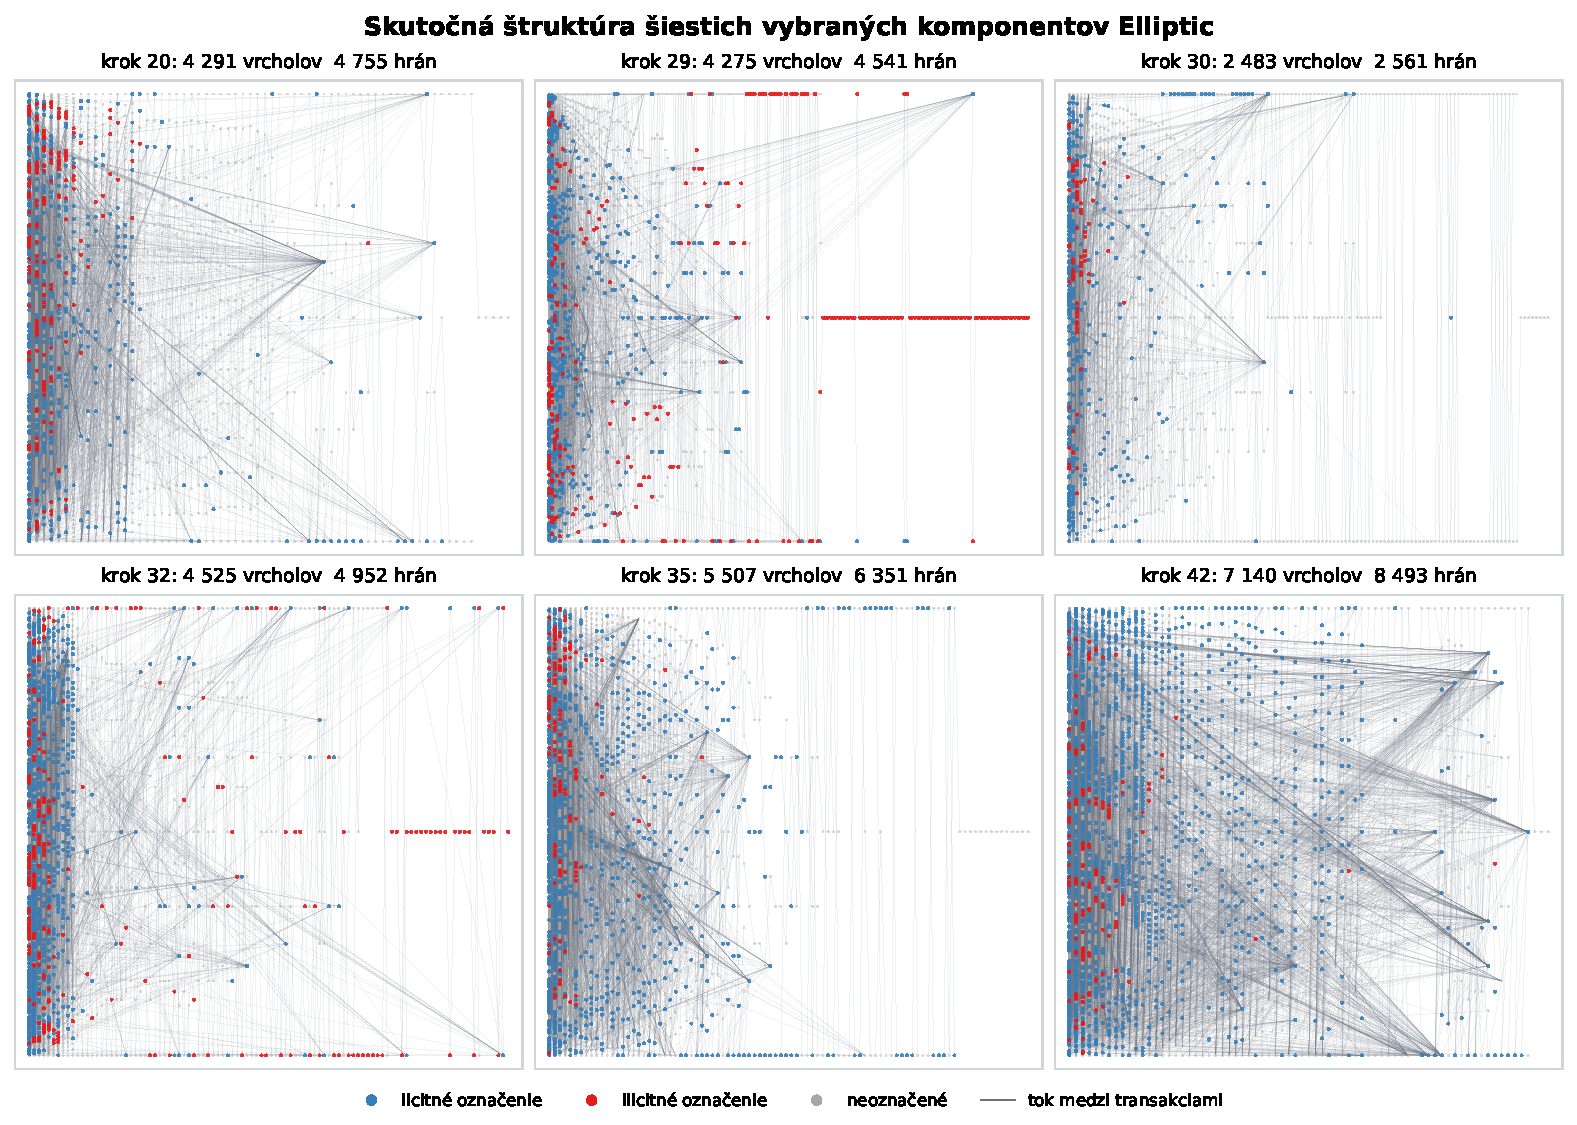
\includegraphics[width=\textwidth]{img/generated/elliptic_graph_overview.pdf}
  \caption[Príklad transakčných podgrafov Elliptic]{Transakčné
  podgrafy časových krokov 20, 29, 30, 32, 35 a 42.
  Body a spojenia predstavujú skutočné záznamy a hrany. Vlastné spracovanie z pôvodných
  súborov Elliptic.}
  \label{fig:elliptic-graph-overview}
  \end{minipage}
\end{center}

\subsection{Prepojenie záznamov s verejným blockchainom}

Interný identifikátor \texttt{txId} spája záznamy v súboroch
Elliptic. Verejný bitcoinový identifikátor \texttt{txid}
má podobu 64 hexadecimálnych znakov a umožňuje vyhľadať konkrétnu
transakciu v blockchaine. Na prechod medzi nimi treba vytvoriť
alebo overiť mapovanie.

Alex Benzik zverejnil mapovanie približne 99,5~\% transakcií
Elliptic~\cite{ellipticMapping}.
Šafář a spoluautori ho použili ako východisko svojho auditu.
Pre známe dvojice získali údaje cez Blockbook a porovnali
vypočítané charakteristiky s číselnými stĺpcami Elliptic.
Takto overovali význam príznakov aj ich väzbu na verejné
záznamy~\cite{safar2026elliptic}.

\begin{center}
  \begin{minipage}{\textwidth}
  \centering
  \captionsetup{type=figure}
  \begin{tikzpicture}
    \node[ellbox,fill=blue!6,text width=32mm,minimum height=19mm]
      (i) at (0,0) {Elliptic\\číselné \texttt{txId}};
    \node[ellbox,fill=black!4,text width=39mm,minimum height=19mm]
      (m) at (4.8,0) {Kandidáti v blokoch\\porovnanie príznakov\\a transakčných väzieb};
    \node[ellbox,fill=blue!6,text width=32mm,minimum height=19mm]
      (h) at (9.6,0) {Verejná transakcia\\64-znakové \texttt{txid}};
    \draw[ellarrow] (i.east) -- (m.west);
    \draw[ellarrow] (m.east) -- (h.west);
  \end{tikzpicture}
  \caption[Mapovanie identifikátorov Elliptic na verejné transakcie]{Mapovanie
  identifikátorov Elliptic na verejné transakcie.
  Porovnanie údajov a transakčných väzieb umožňuje overiť
  zhodu medzi interným záznamom a verejnou transakciou.
  Vlastné spracovanie podľa~\cite{safar2026elliptic}.}
  \label{fig:elliptic-mapping}
  \end{minipage}
\end{center}

Číselné stĺpce okrem časového kroku majú približne nulový priemer
a jednotkovú smerodajnú odchýlku. Autori túto vlastnosť
interpretovali ako výsledok štandardizácie pomocou z-skóre:
\begin{equation}
  z_{ik}=\frac{x_{ik}-\mu_k}{\sigma_k},
  \qquad \sigma_k>0,
  \label{eq:z-score}
\end{equation}
kde $x_{ik}$ označuje pôvodnú hodnotu príznaku $k$
pri transakcii $i$, $\mu_k$ priemer stĺpca a $\sigma_k$
jeho smerodajnú odchýlku.
Po odhade parametrov možno hodnotu previesť späť vzťahom
$x_{ik}=\mu_k+\sigma_k z_{ik}$. Pri celočíselných počtoch
autori využili odstupy medzi hodnotami a pri koreláciách
známe ohraničenie ich rozsahu.

Zo známych transakcií následne odvodili kandidátske bloky
pre každý časový krok. V týchto blokoch prešli transakcie,
vypočítali obnovené príznaky vrátane adresných štatistík
k bloku 575~059 a porovnali ich s denormalizovanými záznamami.
Pri kolíziách rovnakých vektorov priradili identifikátory
podľa pôvodného usporiadania záznamov.
Takéto prípady vyžadujú odlíšenie od zhôd, pri ktorých
charakteristiky určujú jediného kandidáta.

Autori uvádzajú, že identifikovali všetky transakcie a pri
spätnom výpočte dosiahli zhodu všetkých obnovených príznakov.
Úplné mapovanie nezverejnili; v diskusii to odôvodňujú svojím
výkladom licenčných podmienok Elliptic.
Výsledky ich analýzy poskytujú podklad na overovanie zhôd
a rekonštrukciu údajov vo vlastnom riešení.

\subsection{Príznaky transakcií a možnosti ich rozšírenia}

Pôvodný Elliptic obsahuje 94 príznakov označených ako lokálne
a 72 agregovaných príznakov susedných transakcií.
Šafář a spoluautori zistili, že lokálna skupina zahŕňa aj
súhrny histórie vstupných a výstupných adries.
Obnovili význam 151 zo 166 príznakov a ich definície
zdokumentovali v sprievodnom
repozitári~\cite{deanonymizedFeatures}.
Tabuľka~\ref{tab:elliptic-features} rozlišuje zdroje týchto údajov.

\begin{table}[htbp]
  \centering
  \small
  \caption[Skupiny a rozsah obnovených príznakov]{Skupiny príznakov
  a rozsah obnovenej sémantiky podľa auditu~\cite{safar2026elliptic,deanonymizedFeatures}.
  Číslovanie nezahŕňa stĺpec \texttt{txId}.}
  \label{tab:elliptic-features}
  \begin{tabularx}{\textwidth}{lXr}
    \toprule
    Rozsah & Zdroj informácie a príklady & Obnovené \\
    \midrule
    1--22 & časový krok, poplatok, počty a hodnoty vstupov
      a výstupov & 19 z 22 \\
    23--94 & prijatá a odoslaná hodnota, zostatok,
      počet transakcií a životnosť adries & 72 zo 72 \\
    95--166 & hodnoty, bloky, poplatky a počty vstupov
      a výstupov susedných transakcií & 60 zo 72 \\
    \midrule
    spolu & & 151 zo 166 \\
    \bottomrule
  \end{tabularx}
\end{table}

Pri opise transakcií vychádzame z počtov vstupov a výstupov,
ich hodnôt a poplatku vypočítaného podľa vzťahu~\eqref{eq:bitcoin-fee}. Medzi
obnovené príznaky patria minimum, maximum, priemer a smerodajná
odchýlka hodnôt. Pearsonov a Spearmanov koeficient vyjadrujú vzťah
hodnôt k pozičným indexom vstupov alebo výstupov, čím zachytávajú
ich usporiadanie v transakcii. Význam stĺpcov 4, 8 a 16 zostáva neurčený.

Adresné charakteristiky zahŕňajú históriu adries zapojených do transakcie.
Autori identifikovali celkovú prijatú a odoslanú hodnotu, dostupný zostatok,
počty prichádzajúcich a odchádzajúcich transakcií a životnosť adresy.
Každú z týchto vlastností agregujú pre vstupné a výstupné adresy pomocou minima,
maxima, smerodajnej odchýlky, priemeru a Pearsonovho a Spearmanovho koeficientu.
Táto skupina obsahuje 72 príznakov.

Pri susedných transakciách autori obnovili súhrny objemu, výšky bloku, poplatku a
počtov vstupov a výstupov. Počítajú ich osobitne pre predchodcov a nasledovníkov,
pričom do výpočtu zahŕňajú aj transakcie mimo uloženého grafu Elliptic. Význam ďalších
dvanástich príznakov v rozsahoch 113--118 a 149--154 zostáva neurčený.

V tejto práci navrhujeme rozšíriť uvedené skupiny o príznaky odvodené z verejných
blockchainových údajov. Ako kandidátov na zaradenie do vlastného dátového súboru
volíme vek míňaných výstupov, podiel najväčšieho výstupu na celkovej výstupnej hodnote
a počet predchádzajúcich transakcií zapojených adries. Vek výstupov vyjadríme počtom blokov
medzi ich vytvorením a minutím. Týmito príznakmi chceme zachytiť dobu držania prostriedkov,
rozdelenie prevádzanej hodnoty a predchádzajúcu aktivitu adries.

\subsection{Obmedzenia dátového súboru}
\label{sec:elliptic-evaluation}

Audit Šafářa a spoluautorov~\cite{safar2026elliptic}
odhalil, že adresné štatistiky Elliptic zodpovedajú
jedinému referenčnému bloku 575~059. Tento blok nasledoval
až po období zobrazených transakcií. Staršie záznamy tak
obsahujú aj informácie o neskoršej aktivite adries,
ako znázorňuje obrázok~\ref{fig:temporal-leakage}.
Vo vlastnom riešení preto použijeme iba históriu dostupnú
v zvolenom okamihu vyhodnotenia transakcie.

\begin{center}
  \begin{minipage}{\textwidth}
  \centering
  \captionsetup{type=figure}
  \begin{tikzpicture}
    \node[ellbox,fill=blue!6,text width=43mm,minimum height=15mm]
      (tr) at (0,0) {Kroky 1--34\\trénovacie transakcie};
    \node[ellbox,fill=black!4,text width=39mm,minimum height=15mm]
      (te) at (4.7,0) {Kroky 35--49\\testovacie transakcie};
    \node[ellbox,fill=red!5,text width=32mm,minimum height=15mm]
      (f) at (9.4,0) {Blok 575~059\\adresné štatistiky};
    \draw[ellarrow] (-2.2,-1.2) -- (11.25,-1.2);
    \node[ellnote] at (2.2,-1.65) {obdobie transakcií Elliptic};
    \node[ellnote] at (9.4,-1.65) {neskorší referenčný bod};
    \draw[ellarrow,dashed] (f.north) -- (9.4,1.6)
      -- (0,1.6) -- (tr.north);
    \node[ellnote] at (4.7,2.05)
      {neskoršia aktivita adresy vstupuje do staršieho príznaku};
  \end{tikzpicture}
  \caption[Časový únik pri spoločnom referenčnom bloku]{Časový únik
  pri spoločnom referenčnom bloku. Transakcie sú časovo oddelené,
  ale ich adresné príznaky vychádzajú z neskoršej histórie.
  Schéma vyjadruje časové poradie udalostí.
  Vlastné spracovanie podľa~\cite{safar2026elliptic}.}
  \label{fig:temporal-leakage}
  \end{minipage}
\end{center}

Pri návrhu programu určíme, či budeme transakciu vyhodnocovať
po potvrdení, alebo pri spätnej analýze s časovým odstupom.
Podľa tohto rozhodnutia zvolíme rozsah dostupnej histórie.
Informácie o nasledovníkoch zahrnieme do príznakov až vtedy,
keď budú príslušné transakcie v sledovanom okamihu známe.

Ďalším obmedzením sú spoločné adresy v rôznych časových krokoch
(obrázok~\ref{fig:address-leakage}).
Opakované adresné štatistiky môžu modelu pomôcť rozpoznať
adresy, ktoré už pozoroval pri učení.
Vo vlastných experimentoch budeme sledovať výskyt spoločných
adries v trénovacej a testovacej časti aj v pridaných grafových
okolách. Tento prekryv zohľadníme pri hodnotení prenosu modelu
na dovtedy nepozorované adresy.

\begin{center}
  \begin{minipage}{\textwidth}
  \centering
  \captionsetup{type=figure}
  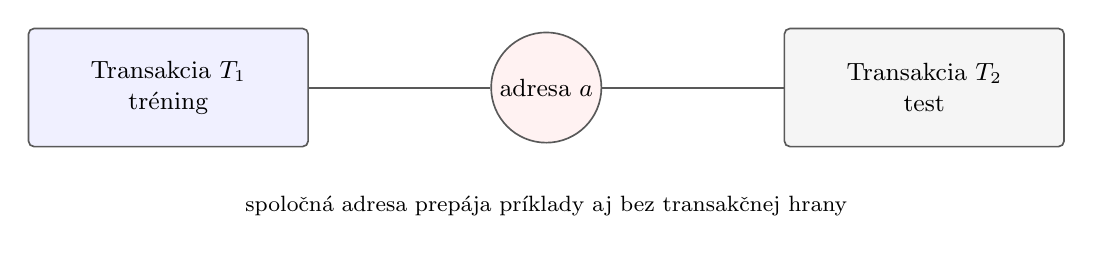
\begin{tikzpicture}
    \node[ellbox,fill=blue!6,text width=32mm,minimum height=15mm]
      (tr) at (0,0) {Transakcia $T_1$\\tréning};
    \node[ellnode,fill=red!5,minimum size=14mm]
      (a) at (4.8,0) {adresa $a$};
    \node[ellbox,fill=black!4,text width=32mm,minimum height=15mm]
      (te) at (9.6,0) {Transakcia $T_2$\\test};
    \draw[draw=black!65,line width=0.7pt] (tr.east) -- (a.west);
    \draw[draw=black!65,line width=0.7pt] (a.east) -- (te.west);
    \node[ellnote] at (4.8,-1.5)
      {spoločná adresa prepája príklady aj bez transakčnej hrany};
  \end{tikzpicture}
  \caption[Prekryv adries medzi tréningom a testom]{Prekryv adries
  medzi tréningom a testom. Úsečky označujú účasť adresy
  v transakcii.
  Vlastné spracovanie podľa~\cite{safar2026elliptic}.}
  \label{fig:address-leakage}
  \end{minipage}
\end{center}

Pôvodná štandardizácia navyše používa priemery a smerodajné
odchýlky celého dátového súboru. Kaufman a spoluautori
aj Kapoor a Narayanan upozorňujú na riziko využívania testovacích
údajov pri príprave modelu~\cite{kaufman2012leakage,kapoor2023leakage}.
Parametre predspracovania odhadneme z trénovacej časti
a v nezmenenej podobe ich použijeme pri spracovaní ostatných
záznamov. Pri interpretácii výsledkov budeme rozlišovať
označenie prevzaté z Elliptic a nezávisle doložený kontext
konkrétnej transakcie. Zverejnené súbory totiž neobsahujú
podklady, podľa ktorých Elliptic priradil entity
k jednotlivým transakciám.

\subsection{Východiská vlastného riešenia}
\label{sec:elliptic-own-approach}

Navrhujeme vytvoriť dátový súbor, v ktorom prepojíme označené
záznamy Elliptic s overenými bitcoinovými transakciami.
Z verejných údajov vypočítame zvolené príznaky a zdokumentujeme
ich význam, jednotku, spôsob výpočtu a rozsah použitej histórie.
Pôvodnú triedu Elliptic zachováme ako cieľové označenie.

Na pripravených údajoch natrénujeme klasifikačný model.
Časť označených transakcií vyhradíme na overenie jeho výsledkov.
Obrázok~\ref{fig:elliptic-own-workflow} oddeľuje učenie
so známymi triedami od použitia modelu na novú transakciu.

\begin{figure}[htbp]
  \centering
  \begin{tikzpicture}
    \node[ellnote,font=\small\bfseries] at (4.8,1.65)
      {A. Príprava dát a učenie modelu};
    \node[ellbox,fill=blue!6,text width=34mm,minimum height=17mm]
      (train) at (0,0) {Trénovacie \texttt{txid}\\triedy Elliptic};
    \node[ellbox,fill=black!4,text width=37mm,minimum height=17mm]
      (features) at (4.8,0) {Verejné údaje\\výpočet príznakov};
    \node[ellbox,fill=blue!6,text width=34mm,minimum height=17mm]
      (fit) at (9.6,0) {Učenie modelu\\príznaky $X$\\triedy $y$};
    \draw[ellarrow] (train.east) -- node[above,ellnote]
      {\texttt{txid}} (features.west);
    \draw[ellarrow] (features.east) -- node[above,ellnote]
      {$X$} (fit.west);
    \draw[ellarrow,dashed] (train.north) -- (0,1.05)
      -- node[above,ellnote] {cieľové triedy $y$} (9.6,1.05) -- (fit.north);

    \node[ellnote,font=\small\bfseries] at (4.8,-1.6)
      {B. Vyhodnotenie novej transakcie};
    \node[ellbox,fill=black!4,text width=34mm,minimum height=17mm]
      (query) at (0,-3.0) {Nové \texttt{txid}\\bez známej triedy};
    \node[ellbox,fill=black!4,text width=37mm,minimum height=17mm]
      (queryfeatures) at (4.8,-3.0) {Verejné údaje\\rovnaké príznaky};
    \node[ellbox,fill=blue!6,text width=34mm,minimum height=17mm]
      (predict) at (9.6,-3.0) {Použitie modelu\\skóre a trieda};
    \draw[ellarrow] (query.east) -- node[above,ellnote]
      {\texttt{txid}} (queryfeatures.west);
    \draw[ellarrow] (queryfeatures.east) -- node[above,ellnote]
      {$\mathbf{x}$} (predict.west);
    \draw[ellarrow,dashed] (fit.south) -- node[right,ellnote,text width=19mm]
      {uložený model} (predict.north);
  \end{tikzpicture}
  \caption[Príprava modelu a vyhodnotenie nového txid]{Oddelenie
  učenia a použitia klasifikačného modelu. Cieľové triedy $y$
  vstupujú do učenia; nová transakcia sa vyhodnotí pomocou rovnakého
  výpočtu príznakov a uloženého modelu. Vlastné spracovanie.}
  \label{fig:elliptic-own-workflow}
\end{figure}

Pre použitie modelu navrhujeme program, do ktorého používateľ
zadá verejné \texttt{txid}. Program získa potrebné údaje,
zopakuje výpočet príznakov a predspracovanie a použije uložený
model. Takto budeme vyhodnocovať aj transakcie mimo učebnej
vzorky, ak budú dostupné všetky požadované vstupy.
Výstupom bude skóre a predikcia triedy; označenie \emph{illicit}
budeme interpretovať ako podnet na ďalšie posúdenie.

% Dočasne vypnuté kapitoly praktickej časti; na obnovenie odstráňte znak %.
%\section{Nástroj BitcoinTxSubgraphBuilder}
\label{sec:safar-tool}

Šafář a spoluautori navrhli otvorený nástroj
\texttt{BitcoinTxSubgraphBuilder}, ktorý z verejných bitcoinových
transakcií zostaví vysvetliteľný dátový súbor. Pri každom príznaku
uchováva jeho význam, postup výpočtu a čas, ku ktorému sa hodnota
vzťahuje \cite{safar2026elliptic,bitcoinSubgraphBuilder}.

Rozbor vychádza zo zdrojového kódu revízie
\texttt{8e01503c0f9f} z 9. februára 2026; úplný identifikátor je uvedený
v bibliografickom zázname repozitára. Jednotlivé podkapitoly sledujú
vstupy, výpočty a uložené výstupy programov. Plný beh vyžaduje vlastný
Bitcoin Core, PostgreSQL, Blockbook, .NET a sekvenčné spracovanie
blockchainu. Praktická časť preto používa menší rozsah; architektúra
pôvodného nástroja určuje kontrolované riziká.

\subsection{Technické pojmy}

\begin{description}
  \item[API] Dohodnutý spôsob, ako si dva programy posielajú požiadavky
  a odpovede. Blockbook API napríklad vráti údaje transakcie podľa
  verejného \texttt{txid}.
  \item[RPC] Rozhranie na volanie funkcie iného programu. Nástroj cez
  Bitcoin Core RPC žiada úplný uzol o bloky a ich transakcie.
  \item[PostgreSQL] Databáza, v ktorej nástroj priebežne uchováva
  transakcie, triedy, vzdialenosti a odpovede Blockbook.
  \item[JSON] Textový formát odpovede API. Obsahuje pomenované polia,
  napríklad \texttt{vin}, \texttt{vout}, \texttt{fees} a
  \texttt{blockHeight}.
  \item[Preskok] Jedna hrana v grafe. Transakcia vo vzdialenosti dva
  preskoky je dostupná cez dve po sebe idúce hrany.
  \item[Parser blockchainu] Program, ktorý číta blok po bloku a mení
  surové transakcie na priebežné štatistiky.
  \item[Kontrolný bod] Súbor s rozpracovaným stavom. Po prerušení možno
  pokračovať od uloženej výšky bloku namiesto opakovania celého výpočtu.
  \item[Stav UTXO] Mapa ešte neminutých výstupov. Umožňuje pri spracovaní
  vstupu nájsť adresu a hodnotu staršieho výstupu.
  \item[Predspracovanie] Posledná úprava dát pred učením, napríklad
  normalizácia čísel a vytvorenie masiek pre tréning, validáciu a test.
\end{description}

\subsection{Čo nástroj rieši a čo potrebuje na vstupe}

Nástroj prijíma zoznam verejných bitcoinových \texttt{txid} s triedami.
Pri práci s Elliptic preto musí existovať samostatné mapovanie
\texttt{txId}$\rightarrow$\texttt{txid}. Anonymizovaný \texttt{txId}
ako vstup nestačí. Nástroj mapovanie nehľadá a neidentifikuje vlastníkov
adries. Spracovanie začína od verejných transakcií, ktoré poskytol
používateľ \cite{safar2026elliptic,bitcoinSubgraphBuilder}.

Obrázok~\ref{fig:safar-tool-architecture} rozdeľuje spracovanie na tri
vrstvy. Modrá časť zhromaždí transakcie a ich grafové okolie. Oranžová
časť prejde blockchain a vytvorí časovo správne štatistiky adries.
Zelená časť spojí oba zdroje do tabuliek použiteľných pri učení.

\begin{figure}[p]
  \centering
  \begin{tikzpicture}[
      >=Latex,
      every node/.style={font=\small,align=center},
      phase/.style={draw,rounded corners=2mm,minimum width=43mm,minimum height=12mm,line width=.7pt},
      store/.style={draw,cylinder,shape border rotate=90,aspect=.23,minimum width=34mm,minimum height=14mm,line width=.7pt},
      flowarrow/.style={-{Latex[length=2.4mm]},line width=.8pt},
      note/.style={font=\scriptsize,align=left,text width=42mm}
    ]
    \node[phase,fill=blue!9] (seed) at (0,0) {označené verejné\\\texttt{txid}};
    \node[phase,fill=blue!9] (import) at (0,-1.8) {Python: import\\počiatočných transakcií};
    \node[phase,fill=blue!9] (expand) at (0,-3.6) {Python: Blockbook\\rozšírenie na $d$ preskokov};
    \node[store,fill=blue!5] (postgres) at (0,-5.6) {PostgreSQL\\transakcie + JSON};

    \node[phase,fill=orange!12] (addresses) at (6.1,-1.8) {C\#: výber adries\\a cieľových výšok};
    \node[phase,fill=orange!12] (scan) at (6.1,-3.6) {C\#: Bitcoin Core\\blok po bloku};
    \node[store,fill=orange!7] (stats) at (6.1,-5.6) {štatistiky adries\\pri každej výške};

    \node[phase,fill=green!10] (construct) at (3.05,-7.7) {C\#: konštrukcia príznakov\\a hrán};
    \node[phase,fill=green!10] (preprocess) at (3.05,-9.5) {Python: predspracovanie\\iba podľa tréningu};
    \node[phase,fill=green!16] (output) at (3.05,-11.3) {CSV + DGL graf\\nový transparentný dátový súbor};

    \draw[flowarrow] (seed) -- (import);
    \draw[flowarrow] (import) -- (expand);
    \draw[flowarrow] (expand) -- (postgres);
    \draw[flowarrow] (postgres.east) to[out=0,in=-90] (addresses.south);
    \draw[flowarrow] (addresses) -- (scan);
    \draw[flowarrow] (scan) -- (stats);
    \draw[flowarrow] (postgres.south) to[out=-90,in=180] (construct.west);
    \draw[flowarrow] (stats.south) to[out=-90,in=0] (construct.east);
    \draw[flowarrow] (construct) -- (preprocess);
    \draw[flowarrow] (preprocess) -- (output);

    \node[note,anchor=west] at (8.6,-2.7)
      {Blockbook poskytne pohodlné\\vyhľadanie konkrétnej transakcie.};
    \node[note,anchor=west] at (8.6,-4.5)
      {Bitcoin Core poskytne úplnú\\chronologickú históriu blokov.};
  \end{tikzpicture}
  \caption{Architektúra nástroja BitcoinTxSubgraphBuilder. Dve vetvy sa
  spoja až pri výpočte príznakov: metadata transakcií pochádzajú z
  Blockbook, časové štatistiky adries zo sekvenčného čítania Bitcoin
  Core. Vlastné spracovanie podľa \cite{safar2026elliptic,bitcoinSubgraphBuilder}.}
  \label{fig:safar-tool-architecture}
\end{figure}

\subsection{Python: vytvorenie transakčného podgrafu}

Prvý program, \texttt{import\_elliptic\_to\_postgres.py}, načíta známe
verejné hashe, triedu a časový krok. Označené transakcie dostanú
vzdialenosť nula. Databázový riadok ďalej obsahuje pole
\texttt{distance}, pôvod v Elliptic a pole \texttt{data}, do ktorého sa
neskôr uloží odpoveď Blockbook.

Druhý program, \texttt{expand\_transaction\_network.py}, buduje okolie
po vrstvách. Z poľa \texttt{vin} číta staršie transakcie, ktorých
výstupy boli minuté. Z poľa \texttt{vout} číta \texttt{spentTxId}, teda
novšie transakcie, ktoré už daný výstup minuli. Okolie sa preto
rozširuje dozadu aj dopredu. Po každej vrstve program stiahne chýbajúce
JSON odpovede a cyklus opakuje, kým vo vzdialenosti najviac $d$ nič
nechýba.

Ak $S$ označuje množinu počiatočných označených transakcií a
$N^{-}(V)$ a $N^{+}(V)$ ich predchodcov a nasledovníkov, vrstvy možno
zapísať takto:
\begin{equation}
  V_0=S,\qquad
  V_k=V_{k-1}\cup N^{-}(V_{k-1})\cup N^{+}(V_{k-1}),
  \quad k=1,\ldots,d.
  \label{eq:hop-expansion}
\end{equation}
Vzdialenosť vrcholu $v$ je dĺžka najkratšej cesty od niektorého
počiatočného vrcholu:
\begin{equation}
  \operatorname{dist}(v,S)=\min_{s\in S}\operatorname{dist}(s,v).
\end{equation}
V praxi sa smer pri meraní okolia ignoruje, hoci vo výslednom grafe sa
smer toku zachováva.

\begin{figure}[htbp]
  \centering
  \begin{tikzpicture}[
      >=Latex,
      every node/.style={font=\small,align=center},
      tx/.style={draw,circle,minimum size=10mm,line width=.7pt},
      edge/.style={-{Latex[length=2mm]},line width=.75pt},
      ring/.style={draw,dashed,rounded corners=3mm,line width=.7pt}
    ]
    \node[ring,minimum width=28mm,minimum height=23mm,fill=green!5] (r0) at (0,0) {};
    \node[ring,minimum width=67mm,minimum height=44mm,fill=blue!3] (r1) at (0,0) {};
    \node[ring,minimum width=105mm,minimum height=64mm,fill=orange!3] (r2) at (0,0) {};
    \node[tx,fill=green!18] (seed) at (0,0) {$S$};
    \node[tx,fill=blue!15] (a) at (-2.1,.9) {$A$};
    \node[tx,fill=blue!15] (b) at (2.1,-.9) {$B$};
    \node[tx,fill=orange!18] (c) at (-4,.3) {$C$};
    \node[tx,fill=orange!18] (d) at (4,1.2) {$D$};
    \node[tx,fill=orange!18] (e) at (3.8,-1.8) {$E$};
    \draw[edge] (c) -- (a);
    \draw[edge] (a) -- (seed);
    \draw[edge] (seed) -- (b);
    \draw[edge] (b) -- (d);
    \draw[edge] (b) -- (e);
    \node[font=\scriptsize,anchor=west] at (5.4,1.4) {$d=2$};
    \node[font=\scriptsize,anchor=west] at (3.6,2.6) {$d=1$};
    \node[font=\scriptsize,anchor=west] at (1.1,1.0) {$d=0$};
  \end{tikzpicture}
  \caption{Rozšírenie podgrafu na dva preskoky. Vrcholy $A$ a $B$ sú
  vzdialené jeden preskok od označenej transakcie $S$; vrcholy $C$,
  $D$ a $E$ dva preskoky. Vlastné spracovanie.}
  \label{fig:hop-expansion}
\end{figure}

Výhoda pevnej vzdialenosti je priamo spojená s grafovým modelom. Sieť
s $L$ vrstvami prijíma správu najviac z $L$ preskokov. Ak dátový súbor
obsahuje okolie do vzdialenosti $d\geq L$, hranica vzorky neodreže
informáciu, ktorú by daný model vedel použiť. Voľba väčšieho $d$
zvyšuje počet vrcholov a pridáva neoznačené kontextové transakcie.

\subsection{C\#: časovo správna história adries}

Samotná odpoveď transakcie neobsahuje úplnú históriu každej adresy v
presnom minulom okamihu. Nástroj preto najprv príkazom
\texttt{extract-addresses} vyberie všetky adresy z podgrafu a ku každej
uloží výšku bloku, pri ktorej bude štatistika potrebná. Príkaz
\texttt{collect} potom číta bloky cez Bitcoin Core RPC od začiatku
reťazca po zadanú cieľovú výšku.

Pri výstupe transakcie analyzátor pridá nový záznam do vlastnej mapy UTXO.
Pri neskoršom vstupe ten istý záznam nájde, prečíta jeho adresu a
hodnotu a z mapy ho odstráni. Tým určí pôvod hodnoty vstupu priamo z
predchádzajúceho výstupu. Počítadlá sa aktualizujú pre adresy potrebné
vo vybranom podgrafe; analyzátor pritom prechádza úplnú chronológiu
blokov.

Pre adresu $a$ a výšku bloku $h$ nástroj uchováva najmä tieto hodnoty:
\begin{align}
  R_a(h) &= \sum_{o:\,\operatorname{addr}(o)=a,\,h(o)\leq h}\operatorname{value}(o),
  &&\text{celková prijatá hodnota},\\
  S_a(h) &= \sum_{i:\,\operatorname{addr}(i)=a,\,h(i)\leq h}\operatorname{value}(i),
  &&\text{celková odoslaná hodnota},\\
  B_a(h) &= R_a(h)-S_a(h),
  &&\text{zostatok},\\
  L_a(h) &= t_a^{\mathrm{last}}(h)-t_a^{\mathrm{first}}(h),
  &&\text{životnosť adresy}.
  \label{eq:address-stats}
\end{align}
Ďalej sa počíta počet transakcií, počet vytvorených výstupov, počet
minutých výstupov a počty prichádzajúcich a odchádzajúcich transakcií.
Hodnota pri $h$ obsahuje iba udalosti s výškou najviac $h$. Transakcia
z budúceho bloku $h+1000$ teda nemôže zmeniť príznak staršej
transakcie pri $h$.

\begin{figure}[htbp]
  \centering
  \begin{tikzpicture}[
      >=Latex,
      every node/.style={font=\small,align=center},
      event/.style={draw,circle,minimum size=9mm,line width=.7pt},
      snapshot/.style={draw,rounded corners=2mm,fill=green!10,minimum width=33mm,minimum height=11mm},
      timearrow/.style={-{Latex[length=2.2mm]},line width=.8pt}
    ]
    \draw[timearrow] (-.5,0) -- (11.2,0) node[right]{výška bloku};
    \node[event,fill=blue!10] (e1) at (1,0) {$h_1$};
    \node[event,fill=blue!10] (e2) at (4,0) {$h_2$};
    \node[event,fill=orange!15] (target) at (7,0) {$h$};
    \node[event,fill=gray!12] (future) at (10,0) {$h+q$};
    \node[snapshot] (state) at (7,-1.7) {príznak pri $h$\\používa $h_1,h_2,h$};
    \draw[timearrow] (e1.south) to[bend right=18] (state.west);
    \draw[timearrow] (e2.south) to[bend right=9] (state.north west);
    \draw[timearrow] (target.south) -- (state.north);
    \draw[dashed,line width=.8pt,red!70] (future.south) to[bend left=20]
      node[below,font=\scriptsize,text=red!70]{nepoužiť} (state.east);
  \end{tikzpicture}
  \caption{Časovo ohraničená štatistika adresy. Budúca udalosť sa do
  príznaku staršej transakcie nezapočíta. Vlastné spracovanie podľa
  \cite{safar2026elliptic,bitcoinSubgraphBuilder}.}
  \label{fig:time-scoped-address-stat}
\end{figure}

Spracovanie celého blockchainu trvá dlho. Implementácia preto sťahuje
bloky do obmedzeného kanála, spracúva ich v poradí a každých 50~000
blokov ukladá stav UTXO aj adresné štatistiky. Prerušený beh možno
obnoviť voľbou \texttt{--checkpoint}. Samostatný príkaz
\texttt{deduplicate} zlúči rovnaké štatistické snímky platné pre viac
cieľových výšok a zmenší výsledný súbor.

\subsection{Konštrukcia príznakov a hrán}

Príkaz \texttt{create-dataset} spojí tri zdroje: JSON transakcie z
PostgreSQL, časové štatistiky adries a hodinovú históriu ceny BTC.
Vytvorí súbor \texttt{tx\_features.csv} a súbor \texttt{edges.csv}.
Hrana sa uloží iba vtedy, keď sa v podgrafe nachádza zdrojová aj cieľová
transakcia. Nesie aj hodnotu minutého výstupu a výšky oboch blokov.

Tabuľka~\ref{tab:open-elliptic-features} uvádza všetky skupiny hodnôt,
ktoré konštruktor počíta. Štatistiky sa počítajú samostatne pre vstupy
a výstupy. Pri každej adresnej vlastnosti sa ukladajú minimum, maximum,
priemer, medián a rozpätie. \emph{Medián} je prostredná hodnota po
zoradení a \emph{rozpätie} je maximum mínus minimum.

\begin{table}[p]
  \centering
  \small
  \caption{Skupiny príznakov vytvárané nástrojom
  BitcoinTxSubgraphBuilder \cite{bitcoinSubgraphBuilder}.}
  \label{tab:open-elliptic-features}
  \begin{tabularx}{\textwidth}{lX}
    \toprule
    Skupina & Význam \\
    \midrule
    základ transakcie & výška bloku, hodnota a hodnota v USD, poplatok
      a poplatok v USD, veľkosť v bajtoch a virtuálnych bajtoch \\
    pomery & poplatok ku vstupnej hodnote, počet vstupov k počtu
      výstupov a počet vstupných transakcií k počtu výstupov \\
    typ transakcie & príznak coinbase a počet vstupných transakcií \\
    opakovanie adries & počet adries spoločných pre vstupy aj výstupy,
      podiel nových výstupných adries a podiel hodnoty smerujúcej na ne \\
    hodnoty vstupov/výstupov & počet, minimum, maximum, smerodajná
      odchýlka, priemer, medián a tie isté sumy po prepočte na USD \\
    podiely hodnôt & minimum, maximum, odchýlka, rozptyl a medián podielu
      jednej položky na celkovej vstupnej alebo výstupnej hodnote \\
    adresy & celkový a jedinečný počet adries a ich vzájomný pomer \\
    história adries & minimum, maximum, priemer, medián a rozpätie pre
      počet transakcií, prichádzajúce a odchádzajúce transakcie,
      zostatok, prijatú hodnotu, odoslanú hodnotu a životnosť \\
    \bottomrule
  \end{tabularx}
\end{table}

Tri odvodené veličiny možno zapísať priamo:
\begin{align}
  r_{\mathrm{fee}} &= \frac{\mathrm{fee}}{\mathrm{valueIn}},\\
  r_{\mathrm{addr}} &=
  \frac{|A_{\mathrm{out}}\setminus A_{\mathrm{in}}|}{|A_{\mathrm{out}}|},\\
  r_{\mathrm{foreign\ value}} &=
  \frac{\sum_{o:\,A(o)\cap A_{\mathrm{in}}=\emptyset}\mathrm{value}(o)}
  {\sum_o\mathrm{value}(o)}.
  \label{eq:open-elliptic-ratios}
\end{align}
Prvý pomer ukazuje, aká časť vstupnej hodnoty tvorí poplatok. Druhý
ukazuje podiel výstupných adries, ktoré sa nenachádzajú medzi vstupmi.
Tretí ukazuje podiel hodnoty odoslanej na takéto adresy. Určenie
vráteného zvyšku vyžaduje ďalšie údaje alebo heuristiku.

Pri kontrole revízie uvedenej na začiatku kapitoly sa našiel aj detail,
ktorý treba pri reprodukcii otestovať: výraz pre
\texttt{VinVoutRatio} delí dve celé čísla pred uložením do typu
\texttt{double}. V jazyku C\# sa tak výsledok najprv skráti na celé
číslo. Ostatný podobný pomer \texttt{TxInVoutRatio} obsahuje explicitný
prevod na \texttt{double}. Táto práca preto nepreberá hodnotu
\texttt{VinVoutRatio} bez samostatného testu a uvádza použitú revíziu
kódu, aby bol výsledok dohľadateľný.

\subsection{Predspracovanie pre strojové učenie}

Surový výstup sa predvolene nenormalizuje. Výskumník tak vidí pôvodné
satoshi, počty a časy a môže ich nezávisle skontrolovať. Voliteľný
skript \texttt{open\_\allowbreak{}elliptic\_\allowbreak{}preprocessing.py}
vytvorí formát podobný Elliptic. Kroky 1--29 používa na tréning, 30--34
na validáciu a 35--49 na test.

Pre každý numerický príznak $j$ sa priemer a smerodajná odchýlka
vypočítajú iba z transakcií dostupných na konci tréningovej časti:
\begin{equation}
  z_{ij}=\frac{x_{ij}-\mu_j^{\mathrm{train}}}
  {\sigma_j^{\mathrm{train}}}.
  \label{eq:safar-train-scaling}
\end{equation}
Rovnaké $\mu_j^{\mathrm{train}}$ a $\sigma_j^{\mathrm{train}}$ sa potom
použijú na validáciu aj test. Skript uloží aj objekt
\texttt{scaler.pkl} s parametrami škálovania, aby sa rovnaká transformácia dala použiť na novej
transakcii. Pri hranách pridá opačný smer pre učenie GNN. Hrany, ktoré
by po obrátení prenášali správu z neskoršej časti do skoršej, odstráni.

\subsection{Presný postup spustenia}

Tabuľka~\ref{tab:safar-commands} oddeľuje príkazy podľa vstupu a
výstupu. Každý krok zodpovedá jednej overiteľnej transformácii dát.

\begin{table}[p]
  \centering
  \scriptsize
  \caption{Postup nástroja podľa dokumentácie a zdrojového kódu
  \cite{bitcoinSubgraphBuilder}.}
  \label{tab:safar-commands}
  \begin{tabularx}{\textwidth}{lXX}
    \toprule
    Krok & Vstup a operácia & Výstup \\
    \midrule
    SQL tabuľky & vytvorenie tabuliek transakcií a adries v PostgreSQL
      & prázdna databázová schéma \\
    import & verejné \texttt{txid}, triedy a časové kroky
      & počiatočné vrcholy so vzdialenosťou 0 \\
    fetch/expand & Blockbook a maximálna vzdialenosť $d$
      & JSON všetkých transakcií podgrafu \\
    extract-addresses & vstupy a výstupy transakcií podgrafu
      & dvojice adresa--cieľová výška \\
    collect & bloky z Bitcoin Core od výšky 0 po cieľ
      & časové snímky štatistík a stav UTXO \\
    deduplicate & opakované rovnaké snímky jednej adresy
      & komprimované štatistiky pre viac výšok \\
    create-dataset & transakcie, štatistiky adries a história ceny
      & \texttt{tx\_features.csv} a \texttt{edges.csv} \\
    predspracovanie & surové CSV a hranice častí
      & normalizované CSV, triedy, hrany a parametre škálovania \\
    prevod do DGL & CSV vo formáte Elliptic
      & binárny graf s príznakmi, triedami a maskami \\
    \bottomrule
  \end{tabularx}
\end{table}

Minimálny logický sled začne importom a rozšírením grafu. Potom sa
extrahujú adresy, zozbierajú a skomprimujú ich štatistiky a napokon sa
vytvorí dátový súbor. Ak sa zmení
maximálna vzdialenosť $d$, zoznam adries alebo cieľová výška, nadväzujúce
výstupy treba vytvoriť znovu alebo jednoznačne oddeliť podľa konfigurácie.

\subsection{Opravené chyby a zostávajúce obmedzenia}

Nástroj zachováva pôvodný význam a jednotku príznakov, adresnú históriu
zastaví pri čase analyzovanej transakcie, normalizáciu učí na
tréningovej časti a grafové okolie vymedzuje
počtom preskokov. Takýto výstup možno vypočítať aj pre novú verejnú
transakciu, čo pri anonymizovaných stĺpcoch pôvodného Elliptic nebolo
možné \cite{safar2026elliptic}.

Nástroj nezaručí nezávislé označenia. Ak trénovacia a
testovacia množina zdieľajú adresu alebo tú istú entitu pod viacerými
adresami, model môže stále rozpoznávať už videný subjekt. Autori preto
odporúčajú vytvoriť nezávislý test, ktorý nezdieľa adresy ani adresy v
$d$-preskokových okoliach. Ani tento technický filter nedokazuje, že dve
odlišné adresy patria rôznym ľuďom.

Ďalším obmedzením je prevádzková náročnosť. Blockbook uľahčuje náhodný
prístup k transakciám; časovo presná história veľkého množstva adries
si vyžaduje sekvenčný prechod blockchainu. Výsledok tiež nemožno
publikovať ako opravený Elliptic, pretože licencia
CC BY-NC-ND 4.0 zakazuje šírenie odvodených upravených verzií. Preto je
potrebné publikovať zdrojový kód, konfiguráciu, verziu vstupov a súhrnné
výsledky. Chránený odvodený dátový súbor sa nezverejňuje
\cite{safar2026elliptic}.

Praktická časť tejto práce používa menší postup. Cez verejný Blockbook
získava šesť časových krokov, odpovede ukladá do SQLite a počíta 18
priamo overiteľných lokálnych príznakov. Bez sekvenčného analyzátora
Bitcoin Core nepočíta úplné časové štatistiky adries. Zvolený rozsah
oddeľuje reprodukovateľný bakalársky experiment od infraštruktúry
potrebnej na tvorbu celého nového dátového súboru.

%\section{Návrh reprodukovateľného experimentu}
\label{sec:methodology}

Experiment je navrhnutý tak, aby bolo možné oddelene skontrolovať
každý krok: výber záznamov, získanie verejnej transakcie, výpočet
príznakov, vytvorenie grafu, rozdelenie dát a trénovanie modelu.
Zdrojový kód sa nachádza v adresári \texttt{analysis/} a poskytuje
príkazy \texttt{prepare}, \texttt{collect}, \texttt{mapping-eval},
\texttt{build-datasets}, \texttt{train} a \texttt{report}.

\subsection{Dátový tok}

Obrázok~\ref{fig:pipeline} ukazuje celý postup. Pôvodné súbory Elliptic
a verejné mapovanie sa najprv obmedzia na vybrané časové kroky. Klient
Blockbook potom získa verejné transakcie a uloží každú úspešnú odpoveď
do databázy SQLite. Z odpovedí sa vypočítajú vysvetliteľné príznaky a
hrany. Posledné dve fázy vytvoria modelové varianty a súhrnné tabuľky
a grafy.

\begin{figure}[htbp]
  \centering
  \resizebox{\textwidth}{!}{%
  \begin{tikzpicture}[
      >=Latex,
      node distance=7mm,
      every node/.style={font=\small,align=center},
      processbox/.style={draw,rounded corners,minimum width=47mm,minimum height=9mm},
      data/.style={processbox,fill=blue!8},
      action/.style={processbox,fill=orange!12}
    ]
    \node[data] (elliptic) {Elliptic + verejné mapovanie};
    \node[action,below=of elliptic] (prepare) {\texttt{prepare}: výber 6 časových krokov};
    \node[action,below=of prepare] (collect) {\texttt{collect}: Blockbook + pamäť SQLite};
    \node[action,below=of collect] (features) {výpočet 18 lokálnych príznakov a hrán};
    \node[action,below left=8mm and 6mm of features] (mapping) {\texttt{mapping-eval}\\skrytých 20~\%};
    \node[action,below right=8mm and 6mm of features] (datasets) {\texttt{build-datasets}\\3 varianty, 2 rozdelenia};
    \node[action,below=18mm of features] (train) {\texttt{train}: LR + RF + GCN};
    \node[data,below=of train] (summary) {\texttt{report}: tabuľky, grafy, manifest};
    \draw[->] (elliptic) -- (prepare);
    \draw[->] (prepare) -- (collect);
    \draw[->] (collect) -- (features);
    \draw[->] (features) -- (mapping);
    \draw[->] (features) -- (datasets);
    \draw[->] (datasets) -- (train);
    \draw[->] (mapping.south) -- (summary.west);
    \draw[->] (train) -- (summary);
  \end{tikzpicture}
  }
  \caption{Dátový tok experimentu. Vlastné spracovanie.}
  \label{fig:pipeline}
\end{figure}

Každý beh vytvorí manifest s cestami a kryptografickými odtlačkami
vstupov, verziou Pythonu a knižníc, počtami záznamov, vybranými krokmi,
rozsahmi blokov a počiatočnou hodnotou generátora náhodných čísel
(angl. \emph{seed}). Surové súbory, mapovanie, vyrovnávacia pamäť API
a odvodený dátový súbor sa neukladajú do systému Git. Dôvodom je veľkosť
údajov aj licencia CC BY-NC-ND 4.0, ktorá obmedzuje ďalšie šírenie
upravených verzií Elliptic \cite{safar2026elliptic,ellipticDataset}.

Tabuľka~\ref{tab:own-pipeline-commands} spresňuje, čo každý príkaz
načíta a čo po sebe zanechá. Takéto oddelenie umožňuje zopakovať iba
zlyhaný krok a súčasne skontrolovať jeho medzivýsledok.

\begin{table}[p]
  \centering
  \small
  \caption{Príkazy vlastného experimentálneho postupu. Vlastné spracovanie.}
  \label{tab:own-pipeline-commands}
  \begin{tabularx}{\textwidth}{lXX}
    \toprule
    Príkaz & Čo vykoná & Kontrolovateľný výstup \\
    \midrule
    \texttt{prepare} & načíta tri súbory Elliptic a verejné mapovanie,
      vyberie šesť krokov a overí identifikátory & vybrané príznaky,
      triedy, hrany, mapovanie a manifest \\
    \texttt{collect} & určí bloky vybraných krokov a cez Blockbook
      načíta všetky kandidátske transakcie & SQLite cache a tabuľka
      transakcií s 18 vypočítanými hodnotami \\
    \texttt{mapping-eval} & skryje 20~\% známych zhôd v každom kroku,
      kalibruje porovnanie iba na zostávajúcich 80~\% & top-1, top-5,
      nejednoznačné a nenájdené prípady \\
    \texttt{build-datasets} & vytvorí tri kombinácie príznakov a grafu,
      časové a adresne oddelené rozdelenie & vrcholy, dve sady hrán a
      masky tréningu, validácie a testu \\
    \texttt{train} & normalizuje podľa tréningu, vyberie hyperparametre
      na validácii a vyhodnotí tri modely & každý beh, metriky, prah a
      agregovaný priemer so smerodajnou odchýlkou \\
    \texttt{report} & číta uložené výsledky bez nového učenia
      & grafy PDF/PNG použité v práci \\
    \bottomrule
  \end{tabularx}
\end{table}

\subsection{Výber časových krokov}

Výber obsahuje dva trénovacie, dva validačné a dva testovacie časové
kroky. Umožňuje zopakovať celý postup na 28~221 vrcholoch bez potreby
spracovať všetkých 203~769 transakcií. Konkrétne počty uvádza
tabuľka~\ref{tab:selected-steps}.

\begin{table}[htbp]
  \centering
  \caption{Vybrané časové kroky a rozdelenie experimentu. Vlastné
  spracovanie z pôvodných súborov Elliptic.}
  \label{tab:selected-steps}
  \begin{tabular}{lrrrrr}
    \toprule
    Časový krok & Časť & Všetky & Licitné & Ilicitné & Neoznačené \\
    \midrule
    20 & tréning & 4~291 & 640 & 260 & 3~391 \\
    29 & tréning & 4~275 & 845 & 329 & 3~101 \\
    30 & validácia & 2~483 & 441 & 83 & 1~959 \\
    32 & validácia & 4~525 & 981 & 342 & 3~202 \\
    35 & test & 5~507 & 1~159 & 182 & 4~166 \\
    42 & test & 7~140 & 1~915 & 239 & 4~986 \\
    \midrule
    Spolu & & 28~221 & 5~981 & 1~435 & 20~805 \\
    \bottomrule
  \end{tabular}
\end{table}

Na obrázku~\ref{fig:selected-split-timeline} je základnou jednotkou
rozdelenia celý časový krok. Vrcholy v rámci kroku sa náhodne nedelia.
Kroky 20 a 29 sú
jediné dáta, z ktorých model upravuje svoje parametre. Kroky 30 a 32
slúžia na výber nastavení a rozhodovacieho prahu. Kroky 35 a 42 sa
použijú až pri konečnom meraní. Medzery medzi číslami pripomínajú, že
výber nepokrýva súvislé obdobie blockchainu.

\begin{figure}[htbp]
  \centering
  \resizebox{\textwidth}{!}{%
  \begin{tikzpicture}[
      >=Latex,
      every node/.style={font=\small,align=center},
      cell/.style={draw,rounded corners,minimum width=23mm,minimum height=14mm}
    ]
    \node[cell,fill=blue!12] (s20) at (0,0) {krok 20\\4~291};
    \node[cell,fill=blue!12] (s29) at (2.7,0) {krok 29\\4~275};
    \node[cell,fill=yellow!20] (s30) at (5.4,0) {krok 30\\2~483};
    \node[cell,fill=yellow!20] (s32) at (8.1,0) {krok 32\\4~525};
    \node[cell,fill=orange!18] (s35) at (10.8,0) {krok 35\\5~507};
    \node[cell,fill=orange!18] (s42) at (13.5,0) {krok 42\\7~140};
    \draw[->,thick] (-1.4,-1.1) -- (14.9,-1.1) node[right]{čas};
    \draw[decorate,decoration={brace,amplitude=5pt,mirror}]
      (-1.1,0.95) -- (3.8,0.95) node[midway,yshift=9mm]{tréning};
    \draw[decorate,decoration={brace,amplitude=5pt,mirror}]
      (4.3,0.95) -- (9.2,0.95) node[midway,yshift=9mm]{validácia};
    \draw[decorate,decoration={brace,amplitude=5pt,mirror}]
      (9.7,0.95) -- (14.6,0.95) node[midway,yshift=9mm]{test};
  \end{tikzpicture}%
  }
  \caption{Časové rozdelenie 28~221 vybraných vrcholov. Číslo pod
  krokom udáva počet všetkých transakcií v danom kroku. Vlastné
  spracovanie z Elliptic.}
  \label{fig:selected-split-timeline}
\end{figure}

Verejné mapovanie obsahuje 28~152 z vybraných 28~221 identifikátorov,
teda 99,76~\% tejto vzorky. Zvyšných 69 záznamov nemá potvrdené
mapovanie. Program pre ne vypíše kandidátov s mierou nejednoznačnosti a
priradí im stav \texttt{candidate\_only}.

\subsection{Zber údajov cez Blockbook}

Blockbook je indexer blockchainu s rozhraním REST. Pre jednu transakciu
vracia okrem \texttt{txid} aj výšku a čas bloku, hodnotu, poplatok,
veľkosť, vstupy a výstupy. Hodnoty sú vyjadrené v najmenšej jednotke
daného blockchainu, pri Bitcoine v satoshi \cite{blockbook}.

Klient používa vlastnú hlavičku \texttt{User-Agent}, časový limit a
exponenciálne predlžovanie prestávky medzi opakovanými pokusmi. Najviac
štyri pracovníky odosielajú požiadavky súbežne, aby sa verejný server
nepreťažoval. Každá odpoveď s kódom 200 sa uloží do SQLite podľa úplnej
adresy požiadavky. Pri opakovanom behu sa teda číta z vyrovnávacej
pamäte a zber môže
pokračovať po prerušení.

Pre vyhodnotenie párovania program prejde všetky transakcie v blokoch
priradených ku konkrétnemu časovému
kroku. Tým vytvorí množinu kandidátov, v ktorej musí algoritmus nájsť
správny verejný \texttt{txid} bez použitia skrytej odpovede.

\subsection{Transparentné lokálne príznaky}

Z jednej odpovede Blockbook sa počíta 18 príznakov so známym významom.
Príznak je číselná hodnota, ktorou sa transakcia opíše modelu.
Samostatné číslo neurčuje triedu; model hľadá kombinácie viacerých
čísel. Tabuľka~\ref{tab:transparent-features} uvádza všetkých 18
hodnôt, ich jednotku a význam.

\begin{table}[p]
  \centering
  \scriptsize
  \caption{Transparentne vypočítané lokálne príznaky.}
  \label{tab:transparent-features}
  \begin{tabularx}{\textwidth}{r l l X}
    \toprule
    Č. & Príznak & Jednotka & Čo model dostane \\
    \midrule
    2 & objem & satoshi & súčet všetkých výstupov transakcie \\
    3 & poplatok & satoshi & vstupná hodnota mínus výstupná hodnota \\
    5 & počet vstupov & počet & koľko starších výstupov sa míňa \\
    6 & počet výstupov & počet & koľko nových výstupov vzniká \\
    7 & jedinečné vstupné adresy & počet & počet rôznych neprázdnych adries vo vstupoch \\
    9 & minimum vstupov & satoshi & najmenší vstup \\
    10 & maximum vstupov & satoshi & najväčší vstup \\
    11 & odchýlka vstupov & satoshi & rozdielnosť veľkostí vstupov \\
    12 & priemer vstupov & satoshi & priemerná hodnota jedného vstupu \\
    13 & Pearson vstupov & $[-1,1]$ & lineárny trend hodnôt podľa indexu \\
    14 & Spearman vstupov & $[-1,1]$ & rast alebo pokles poradia hodnôt \\
    15 & jedinečné výstupné adresy & počet & počet rôznych neprázdnych adries vo výstupoch \\
    17 & minimum výstupov & satoshi & najmenší výstup \\
    18 & maximum výstupov & satoshi & najväčší výstup \\
    19 & odchýlka výstupov & satoshi & rozdielnosť veľkostí výstupov \\
    20 & priemer výstupov & satoshi & priemerná hodnota jedného výstupu \\
    21 & Pearson výstupov & $[-1,1]$ & lineárny trend hodnôt podľa indexu \\
    22 & Spearman výstupov & $[-1,1]$ & rast alebo pokles poradia hodnôt \\
    \bottomrule
  \end{tabularx}
\end{table}

Pri príklade z obrázka~\ref{fig:utxo-example} by počet vstupov bol 2,
počet výstupov 2, minimum vstupov 0,4 BTC, maximum vstupov 0,6 BTC,
priemer vstupov 0,5 BTC a poplatok 0,01 BTC. Počet jedinečných adries
sa môže od počtu vstupov líšiť, pretože jedna adresa sa môže objaviť
viackrát. Program najprv vytvorí množinu adries a až potom ju spočíta.

Pri prázdnej postupnosti, napríklad pri vstupoch coinbase transakcie,
sa agregačná hodnota nastaví na nulu. Smerodajná odchýlka jednej
hodnoty a korelácia konštantnej postupnosti sú tiež nula. Toto pravidlo
je súčasťou implementácie a testov, pretože matematická korelácia v
takých prípadoch nie je určená.

\subsection{Kontrolovaný experiment párovania}

Verejné mapovanie už obsahuje známe odpovede. Presnosť metódy sa preto
meria po skrytí 20~\% známych dvojíc v každom zo šiestich časových
krokov pomocou \texttt{seed=42}. Zvyšných 80~\% slúži na
odhad lineárneho prevodu medzi normalizovaným príznakom Elliptic a
hodnotou vypočítanou z blockchainu:
\begin{equation}
  \hat{x}=a z+b.
\end{equation}
Koeficienty $a$ a $b$ sa určia metódou najmenších štvorcov. Skryté
\texttt{txid} sa nepoužijú pri odhade ani pri tvorbe kandidátov.

Vyhľadávanie sa hodnotí v troch stupňoch:
\begin{enumerate}
  \item iba počet vstupov a výstupov;
  \item počty doplnené o objem, poplatok a počty jedinečných adries;
  \item všetkých 18 obnovených lokálnych príznakov.
\end{enumerate}
Najprv sa kandidáti zúžia na rovnaký počet vstupov a výstupov. Potom
sa zoradia podľa priemernej normalizovanej absolútnej odchýlky ostatných
príznakov. Zaznamenáva sa úspešnosť top-1 a top-5, počet kandidátov,
chýbajúce výsledky a prípady, keď dvaja kandidáti dosiahnu rovnaké
skóre. Takéto prípady sa označia ako nejednoznačné.

\subsection{Varianty dát a grafu}

Experiment porovnáva tri varianty:
\begin{enumerate}[label=\Alph*.]
  \item pôvodné anonymizované príznaky a pôvodný graf Elliptic;
  \item transparentné lokálne príznaky a pôvodný graf Elliptic;
  \item transparentné lokálne príznaky a graf rekonštruovaný z odkazov
  vstupov na staršie \texttt{txid}.
\end{enumerate}

Variant B oddeľuje vplyv príznakov, kým rozdiel medzi B a C oddeľuje
vplyv grafu. Logistická regresia a náhodný les graf nepoužívajú, preto
pri nich varianty B a C slúžia ako kontrola a musia pri rovnakej
počiatočnej hodnote
poskytnúť rovnaký výsledok. Pri GCN sa graf priamo podieľa na výpočte
reprezentácie vrcholu.

Podobný dôraz na vopred určené rozdelenia, spoločný formát vstupu a
jednotný hodnotiaci postup používa aj Open Graph Benchmark. Jeho
autori zdôrazňujú, že rozdelenie má napodobniť konkrétne budúce
použitie modelu. Náhodné percentá riadkov túto požiadavku nespĺňajú
\cite{hu2020ogb}. Pre túto prácu z toho vyplýva, že názov algoritmu bez
opisu času, grafových hrán a spoločných adries nestačí na porovnanie.

\subsection{Časové rozdelenie a rozdelenie odolné voči úniku informácií}

Bežné časové rozdelenie priradí celé kroky 20 a 29 do tréningu, kroky
30 a 32 do validácie a kroky 35 a 42 do testu. Tým sa do rôznych častí
náhodne nerozdelia vrcholy jedného časového komponentu Elliptic. Adresa
\texttt{A} sa napriek tomu môže objaviť v trénovacej
transakcii a znova v testovacej transakcii. Model potom môže využiť
opakovanú entitu.

Druhé rozdelenie sa tvorí postupne zľava doprava. Najprv sa prijmú
trénovacie transakcie a zapamätajú sa všetky ich vstupné a výstupné
adresy. Validačná transakcia sa prijme iba vtedy, keď nepoužíva žiadnu
zapamätanú adresu. Jej adresy sa potom tiež zapamätajú. Rovnaké pravidlo
sa nakoniec použije na test. Tento postup zachováva opakovania adresy
v rámci jednej časti a vylúči jej výskyt v neskoršej časti.

\begin{figure}[htbp]
  \centering
  \begin{tikzpicture}[
      >=Latex,
      node distance=7mm,
      every node/.style={font=\small,align=center},
      box/.style={draw,rounded corners,minimum width=40mm,minimum height=11mm}
    ]
    \node[box,fill=blue!12] (train) {tréning\\ulož adresy $\{A,B\}$};
    \node[box,right=of train,fill=yellow!20] (val) {validácia\\odstráň riadok s $A$};
    \node[box,right=of val,fill=orange!18] (test) {test\\odstráň riadok s $A,B$};
    \draw[->] (train) -- node[above,font=\scriptsize]{zakázané v ďalšej časti} (val);
    \draw[->] (val) -- node[above,font=\scriptsize]{rozšírený zoznam} (test);
    \node[box,below=12mm of val,fill=gray!10,minimum width=48mm]
      (edges) {nakoniec odstráň hrany\\medzi rozdielnymi časťami};
    \draw[->] (train.south) -- (edges.west);
    \draw[->] (val.south) -- (edges.north);
    \draw[->] (test.south) -- (edges.east);
  \end{tikzpicture}
  \caption{Tvorba rozdelenia bez pozorovateľného prekryvu adries.
  Písmená $A$ a $B$ sú ilustračné adresy. Vlastné spracovanie.}
  \label{fig:clean-split-process}
\end{figure}

Po filtrovaní vrcholov sa odstránia aj všetky hrany, ktorých konce
patria do rozdielnych častí. GCN preto nemôže preniesť informáciu z
trénovacieho vrcholu do validačného alebo testovacieho vrcholu.
Transakcie bez overeného verejného mapovania sa do tohto rozdelenia
nezaradia, pretože pri nich nemožno spoľahlivo skontrolovať adresy.
Počty vyradených vrcholov sa uvádzajú spolu s výsledkami; metrika po
filtrovaní totiž vzniká na menšej a odlišnej vzorke.

Pri variante A zostáva časový únik ukrytý v pôvodných adresných
príznakoch 23--94. Rozdelenie odstraňuje pozorovateľný prekryv adries a
hrán medzi časťami. Informácia z budúcnosti už zapísaná v jednom
vektore zostáva zachovaná. Transparentné varianty B a C tieto globálne
adresné príznaky nepoužívajú.

\subsection{Modely a hyperparametre}

Experiment používa tri referenčné algoritmy ako kontrolné body:
lineárny model, nelineárny tabuľkový model a model využívajúci graf.
Práca nepripisuje týmto algoritmom vlastný metodický prínos. Ak bude v
ďalšej verzii práce vytvorený vlastný
klasifikátor, musí sa porovnať na rovnakých vstupoch, rozdeleniach a
metrikách. Číslo prevzaté z experimentu s inými podmienkami neposkytuje
porovnateľný základ.

\begin{table}[htbp]
  \centering
  \small
  \caption{Presné algoritmy použité v implementácii. Vlastné spracovanie.}
  \label{tab:implemented-models}
  \begin{tabularx}{\textwidth}{lXX}
    \toprule
    Model & Implementácia & Čo sa počas učenia mení \\
    \midrule
    logistická regresia &
      \texttt{LogisticRegression} z knižnice scikit-learn,
      vyvážené váhy tried, najviac 2~000 iterácií &
      jedna váha pre každý príznak a posun $b$; validácia vyberá
      $C\in\{0{,}1;1;10\}$ a rozhodovací prah \\
    náhodný les &
      \texttt{RandomForestClassifier} z knižnice scikit-learn,
      500 stromov &
      otázky v uzloch stromov; validácia vyberá hĺbku 10, 20 alebo bez
      limitu a minimálne 1 alebo 5 vzoriek v liste \\
    dvojvrstvová GCN &
      vlastná trieda v PyTorch, dve lineárne vrstvy 128$\rightarrow$2,
      riedka normalizovaná matica susednosti &
      matice váh oboch vrstiev; Adam používa krok 0,01, váhový útlm
      $5\cdot10^{-4}$, dropout 0,5 a skoré zastavenie po 8 epochách \\
    \bottomrule
  \end{tabularx}
\end{table}

Váhy neurónového a lineárneho modelu sa všeobecne menia proti smeru,
v ktorom rastie stratová funkcia:
\begin{equation}
  \boldsymbol{\theta}_{t+1}
  =\boldsymbol{\theta}_{t}-\eta\nabla_{\boldsymbol{\theta}}
  \mathcal{L}(\boldsymbol{\theta}_{t}),
  \label{eq:gradient-update}
\end{equation}
kde $\boldsymbol{\theta}$ označuje učené parametre, $\eta$ rýchlosť
učenia a $\nabla\mathcal{L}$ smer najväčšieho rastu chyby. V praxi GCN
používa adaptívny algoritmus Adam, ktorý pre každý parameter upravuje
veľkosť kroku podľa priebehu predchádzajúcich gradientov. Náhodný les
gradient nepoužíva; skladá rozhodovacie pravidlá priamo z trénovacích
príkladov.

Pred učením sa každý príznak prevedie na porovnateľnú mierku. Ak sú
napríklad poplatky v tisícoch satoshi a korelácia v intervale
$[-1,1]$, veľké jednotky poplatku by mohli neprimerane ovplyvniť
optimalizáciu. Štandardizovaná hodnota je
\begin{equation}
  z_{ij}=\frac{x_{ij}-\mu_j^{\mathrm{train}}}
  {\sigma_j^{\mathrm{train}}},
  \label{eq:training-standardization}
\end{equation}
kde $x_{ij}$ je príznak $j$ transakcie $i$. Priemer $\mu_j$ a
smerodajná odchýlka $\sigma_j$ sa počítajú výhradne z tréningu.
Validácia a test používajú tie isté trénovacie hodnoty. Model tak pri
príprave vstupu nevidí rozdelenie budúcich dát.

\subsubsection{Logistická regresia}

Logistická regresia priradí každému príznaku váhu. Kladná váha zvyšuje
skóre ilicitnej triedy, záporná ho
znižuje a váha blízka nule znamená malý lineárny vplyv. Pre vektor
príznakov $\mathbf{x}$ najprv vypočíta
\begin{equation}
  s=\mathbf{w}^{\mathsf T}\mathbf{x}+b,
\end{equation}
kde $\mathbf{w}$ sú učené váhy a $b$ je posun. Sigmoidálna funkcia
prevedie neobmedzené skóre na číslo od 0 do 1:
\begin{equation}
  p(y=1\mid\mathbf{x})=\frac{1}{1+\mathrm{e}^{-s}}.
  \label{eq:logistic-sigmoid}
\end{equation}
Ak je napríklad výsledok 0,82, model priradil transakcii skóre 0,82
pre ilicitnú triedu. Skóre je výstup modelu kalibrovaného voči
označeniam Elliptic a nemá význam právnej pravdepodobnosti.

Počas učenia sa váhy menia tak, aby znižovali binárnu krížovú entropiu
\begin{equation}
  \mathcal{L}=-\frac{1}{n}\sum_{i=1}^{n}
  \left[y_i\log p_i+(1-y_i)\log(1-p_i)\right].
\end{equation}
Sebavedomá chybná predikcia vytvorí veľkú stratu. Regularizácia bráni
neprimerane veľkým váham. Implementácia porovnáva
$C\in\{0{,}1;1;10\}$ a vyberá hodnotu podľa validačného $F_1$.
Váhy tried sú vyvážené, aby početnejšia licitná trieda nepotlačila
menšiu ilicitnú triedu.

\subsubsection{Náhodný les}

Rozhodovací strom sa učí sériu otázok typu \uv{je poplatok menší než
hranica $t$?} alebo \uv{je počet výstupov väčší než 2?}. Každá otázka
rozdelí trénovacie príklady na dve vetvy. Algoritmus vyberá príznak a
hranicu, ktoré znižujú nečistotu tried. Giniho nečistota uzla je
\begin{equation}
  G=1-\sum_{k\in\{0,1\}}p_k^2,
  \label{eq:gini}
\end{equation}
kde $p_k$ je podiel triedy $k$ v uzle. Ak uzol obsahuje iba jednu
triedu, $G=0$. Pri rovnakom zastúpení dvoch tried je $G=0{,}5$.

Jeden strom sa môže príliš prispôsobiť náhodným detailom tréningu.
Náhodný les preto vytvorí 500 stromov. Každý strom dostane náhodnú
vzorku trénovacích riadkov a pri delení skúma náhodnú podmnožinu
príznakov. Výsledné skóre je priemer hlasov stromov. Model tak dokáže
zachytiť nelineárne pravidlá, napríklad kombináciu nízkeho počtu
výstupov, vysokej hodnoty a nezvyčajného poplatku
\cite{breiman2001random}.

Ak $p_m(y=1\mid\mathbf{x})$ je podiel ilicitných trénovacích príkladov
v liste stromu $m$, skóre celého lesa s $M=500$ stromami je
\begin{equation}
  p_{\mathrm{RF}}(y=1\mid\mathbf{x})
  =\frac{1}{M}\sum_{m=1}^{M}p_m(y=1\mid\mathbf{x}).
  \label{eq:rf-average}
\end{equation}
Les teda nehľadá jednu jedinú charakteristiku \uv{ilicitnosti}. Každý
strom vytvorí inú postupnosť otázok a konečné skóre ich spriemeruje.

Porovnávajú sa maximálne hĺbky 10, 20 a bez obmedzenia a minimálne
počty vzoriek v liste 1 alebo 5. Najlepšia kombinácia sa zvolí na
validácii pri počiatočnej hodnote 42. Potom sa celý les naučí päťkrát
s hodnotami 42 až 46. Rozdiel medzi behmi ukazuje, ako výsledok závisí
od náhodného výberu vzoriek a príznakov.

\subsubsection{Grafová konvolučná sieť}

Logistická regresia a náhodný les posudzujú každý riadok samostatne.
Grafová konvolučná sieť (GCN) doplní k príznakom transakcie aj
informáciu od jej susedov. Pred výpočtom sa ku každému vrcholu pridá
hrana do seba a matica susednosti sa normalizuje:
\begin{equation}
  \hat{A}=A+I,\qquad
  \tilde{A}=\hat{D}^{-1/2}\hat{A}\hat{D}^{-1/2}.
\end{equation}
Matica $A$ opisuje hrany, $I$ pridáva vlastnú informáciu vrcholu a
$\hat{D}$ obsahuje počty spojení. Normalizácia bráni tomu, aby vrchol s
mnohými susedmi získal automaticky neúmerne veľké hodnoty.

Jedna grafová vrstva sa dá zapísať ako
\begin{equation}
  H^{(l+1)}=\sigma\!\left(\tilde{A}H^{(l)}W^{(l)}\right),
  \label{eq:gcn-layer}
\end{equation}
kde $H^{(0)}=X$ je vstupná matica príznakov, $W^{(l)}$ sú učené váhy a
$\sigma$ je aktivačná funkcia. Prvá vrstva v implementácii vytvorí pre
každý vrchol 128 skrytých hodnôt. Použitá funkcia ReLU ponechá kladné
číslo a záporné nahradí nulou:
\begin{equation}
  \operatorname{ReLU}(z)=\max(0,z).
  \label{eq:relu}
\end{equation}
Nelinearita umožňuje dvom vrstvám modelovať vzťahy, ktoré jedna
lineárna transformácia nezachytí. Po ReLU sa počas tréningu náhodne vynuluje polovica
skrytých hodnôt. Tento postup sa nazýva náhodné vypínanie, angl.
\emph{dropout}. Model sa tým učí používať viac skrytých hodnôt.

Druhá grafová vrstva vytvorí dve skóre, jedno pre licitnú a druhé pre
ilicitnú triedu. Funkcia softmax ich prevedie na súčet 1:
\begin{equation}
  p_k=\frac{\mathrm{e}^{s_k}}
  {\mathrm{e}^{s_0}+\mathrm{e}^{s_1}},\qquad k\in\{0,1\}.
  \label{eq:softmax}
\end{equation}
Váhy sa
upravujú algoritmom Adam s rýchlosťou učenia 0,01 a váhovým útlmom
$5\cdot10^{-4}$. Používa sa vážená krížová entropia, aby ilicitná
trieda mala napriek menšiemu počtu príkladov primeraný vplyv. Tréning
má najviac 200 epoch; epocha je jeden úplný krok učenia nad
trénovacími vrcholmi. Ak sa validačný $F_1$ nezlepší osem epoch, uloží
sa najlepší skorší stav a učenie sa zastaví \cite{kipf2017gcn}.

Dve grafové vrstvy znamenajú, že reprezentácia vrcholu môže obsahovať
informáciu od susedov vzdialených najviac dva preskoky. Neoznačené
vrcholy zostávajú v grafe a môžu sprostredkovať túto informáciu. Keďže
nemajú cieľovú triedu, nevstupujú do stratovej funkcie ani do metrík.

\subsubsection{Spoločný postup učenia}

\begin{figure}[htbp]
  \centering
  \resizebox{\textwidth}{!}{%
  \begin{tikzpicture}[
      >=Latex,
      node distance=6mm,
      every node/.style={font=\small,align=center},
      flowbox/.style={draw,rounded corners,minimum width=31mm,minimum height=13mm}
    ]
    \node[flowbox,fill=blue!10] (train) {tréning\\uprav váhy};
    \node[flowbox,right=of train,fill=yellow!18] (validation) {validácia\\vyber nastavenia a prah};
    \node[flowbox,right=of validation,fill=green!10] (freeze) {uzamkni model\\už nič neuč};
    \node[flowbox,right=of freeze,fill=orange!16] (test) {test\\zmeraj výsledok raz};
    \draw[->] (train) -- (validation);
    \draw[->] (validation) edge[bend left=22] node[above,font=\scriptsize]{ďalšie nastavenie} (train);
    \draw[->] (validation) -- (freeze);
    \draw[->] (freeze) -- (test);
  \end{tikzpicture}%
  }
  \caption{Oddelenie učenia, výberu nastavení a konečného testu.
  Testovacie dáta sa nevracajú späť do učenia. Vlastné spracovanie.}
  \label{fig:model-training-flow}
\end{figure}

Každý model vráti skóre ilicitnej triedy od 0 do 1. Na validácii sa
skúšajú prahy od 0,05 do 0,95 s krokom 0,01 a vyberie sa prah s
najvyšším ilicitným $F_1$. Ak je napríklad prah 0,63, skóre 0,70 sa
zmení na ilicitnú predikciu a skóre 0,40 na licitnú. Vybraný prah sa
bez ďalšej úpravy použije na test.

\subsection{Metriky a interpretačné pravidlá}

Predikcie sa najprv rozdelia do štyroch skupín. \emph{TP} je správne
zachytená ilicitná transakcia. \emph{FP} je licitná transakcia, ktorú
model omylom označil ako ilicitnú. \emph{FN} je nezachytená ilicitná
transakcia a \emph{TN} je správne rozpoznaná licitná transakcia. Tieto
štyri počty tvoria maticu zámen.

Precíznosť odpovedá na otázku: \uv{Ak model upozornil na transakciu,
ako často mal podľa dát pravdu?}
\begin{equation}
  \mathrm{precision}=\frac{TP}{TP+FP}.
\end{equation}
Úplnosť odpovedá na inú otázku: \uv{Koľko zo všetkých ilicitných
transakcií model našiel?}
\begin{equation}
  \mathrm{recall}=\frac{TP}{TP+FN}.
\end{equation}
Označenie väčšieho počtu transakcií môže zvýšiť úplnosť a súčasne
vytvoriť viac falošných upozornení. Hlavná metrika $F_1$ je
harmonický priemer oboch hodnôt:
\begin{equation}
  F_1 = 2\frac{\mathrm{precision}\cdot\mathrm{recall}}
  {\mathrm{precision}+\mathrm{recall}}.
\end{equation}

Ak je napríklad $TP=80$, $FP=20$ a $FN=40$, precíznosť je
$80/(80+20)=0{,}80$, úplnosť $80/(80+40)=0{,}67$ a $F_1$ približne
0,73. Vysoká obyčajná presnosť by bola pri nevyvážených triedach
zavádzajúca: model by mohol označiť všetko ako licitné a napriek tomu
správne zaradiť väčšinu riadkov.

Vyvážená úspešnosť je priemer správne zachyteného podielu licitnej a
ilicitnej triedy. PR-AUC je plocha pod krivkou precíznosti a úplnosti
pri všetkých možných prahoch. Hodnotí poradie skóre bez výberu jediného
prahu. Hodnota smerujúca k 1 je
lepšia; jej základná úroveň závisí od podielu ilicitnej triedy.

Výsledok modelu sa interpretuje ako predikcia triedy v dátovom súbore
a neposkytuje dôkaz trestného činu. Kandidát párovania vyjadruje
technickú podobnosť s verejnou transakciou bez identifikácie osoby.

%\section{Overenie dát a vyhodnotenie}
\label{sec:results}

Výsledky zahŕňajú kontrolu vstupných súborov, párovanie a klasifikáciu.
Pri každom výsledku sa rozlišuje priamo overená zhoda, experimentálny
kandidát a obmedzenie použitej metódy.

\subsection{Kontrola vybranej vzorky}

Program načítal pôvodný súbor 203~769 vrcholov po častiach a ponechal
časové kroky 20, 29, 30, 32, 35 a 42. Výsledných 28~221 vrcholov je
spojených 31~653 hranami pôvodného grafu. Súčet tried v každom kroku
zodpovedá počtu vrcholov uvedenému v tabuľke~\ref{tab:selected-steps}.

Z vybraných vrcholov má 7~416 známu triedu a 20~805 je neoznačených.
Medzi známymi triedami je 5~981 licitných a 1~435 ilicitných označení.
Obrázok~\ref{fig:selected-distribution} ukazuje výraznú triednu
nevyváženosť aj rozdielnu veľkosť časových krokov. Hodnotenie preto
používa aj metriky zamerané na menej početnú ilicitnú triedu.

\begin{figure}[htbp]
  \centering
  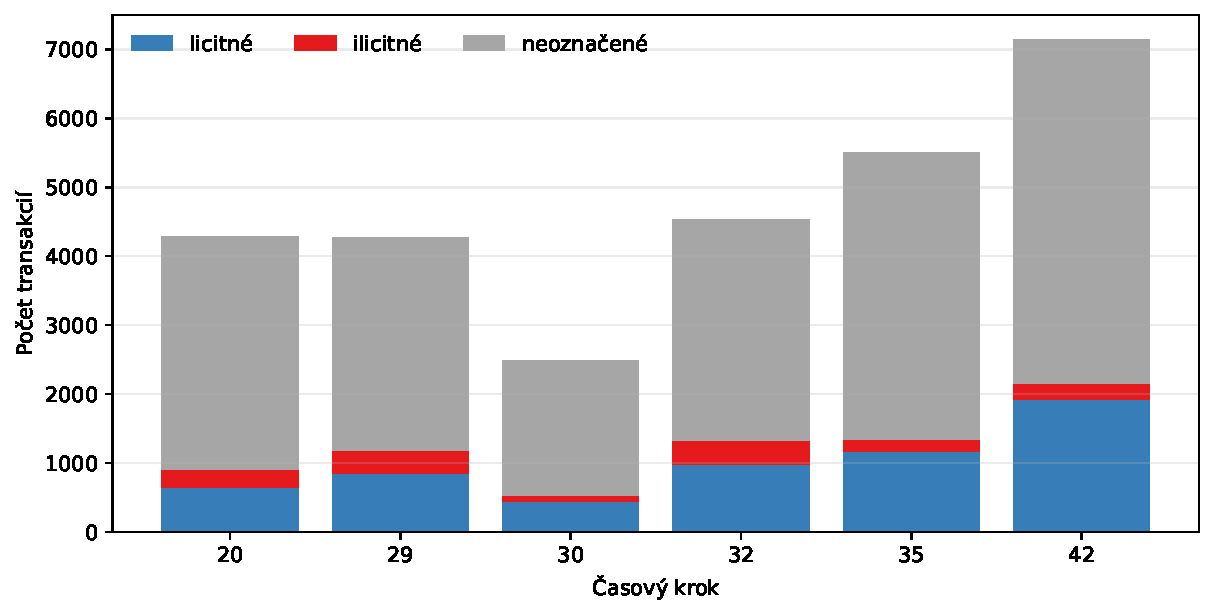
\includegraphics[width=0.9\textwidth]{img/generated/elliptic_class_distribution.pdf}
  \caption{Rozdelenie tried vo vybraných časových krokoch. Vlastné
  spracovanie z pôvodných súborov Elliptic.}
  \label{fig:selected-distribution}
\end{figure}

Verejné mapovanie obsahuje 28~152 z 28~221 vybraných záznamov. Kontrola
formátu overuje, že každý verejný identifikátor má hexadecimálny tvar a
že jeden anonymizovaný identifikátor sa vo výbere nevyskytuje viackrát.
Zvyšných 69 záznamov ostáva bez potvrdeného verejného \texttt{txid}.

\subsection{Kontrola zberu a výpočtu príznakov}

Živá skúška klienta Blockbook overuje načítanie transakcie aj celého
bloku. Pri transakcii sa kontroluje rovnosť medzi poplatkom z odpovede
a rozdielom súčtu vstupov a výstupov, ak sú obe hodnoty dostupné.
Jednotkové testy pokrývajú prevod BTC na satoshi, počet vstupov a
výstupov, jedinečné adresy, coinbase transakciu, rekonštrukciu hrán a
opätovné načítanie odpovede z vyrovnávacej pamäte SQLite.

Ilustračný príklad z obrázka~\ref{fig:utxo-example} má vstupy 0,6 a
0,4 BTC, výstupy 0,8 a 0,19 BTC a vypočítaný poplatok 0,01 BTC. Tento
malý príklad je súčasne testom, že program nezamieňa objem výstupov za
hodnotu vstupov a že poplatok nevytvára ako samostatný výstup.

\subsection{Výsledky párovania}

Z 28~152 známych zhôd bolo vopred skrytých 5~630 záznamov, teda 20~\%
v každom časovom kroku po zaokrúhlení. Množina kandidátov obsahovala
97~533 verejných transakcií zo všetkých 62 zvolených blokov. Správna
transakcia bola pre každý skrytý záznam v dostupnom rozsahu blokov;
počet prípadov bez kandidáta bol preto vo všetkých stupňoch nulový.

\begin{table}[htbp]
  \centering
  \caption{Výsledky párovania na skrytých známych záznamoch. Vlastné
  spracovanie.}
  \label{tab:mapping-results}
  \begin{tabular}{lrrrr}
    \toprule
    Použité príznaky & Top-1 & Top-1 [\%] & Top-5 [\%] & Nejednoznačné \\
    \midrule
    počty vstupov a výstupov & 151 & 2,68 & 5,60 & 5~545 \\
    počty, hodnoty, poplatok a adresy & 5~513 & 97,92 & 99,47 & 166 \\
    všetkých 18 lokálnych príznakov & 5~593 & 99,34 & 99,79 & 50 \\
    \bottomrule
  \end{tabular}
\end{table}

Počty vstupov a výstupov sú slabým identifikátorom, pretože
mnohé transakcie majú rovnakú základnú štruktúru. Po pridaní objemu,
poplatku a jedinečných adries vzrástla top-1 úspešnosť na 97,92~\%.
Úplný lokálny vektor dosiahol 99,34~\%. Zostávajúce kolízie vznikli pri
podobných alebo zhodných vektoroch a pri chybe lineárnej rekonštrukcie.
Pre 69 pôvodne nezmapovaných záznamov sa preto uvádza zoznam kandidátov;
žiadny z nich sa neoznačuje ako potvrdená zhoda.

\begin{figure}[htbp]
  \centering
  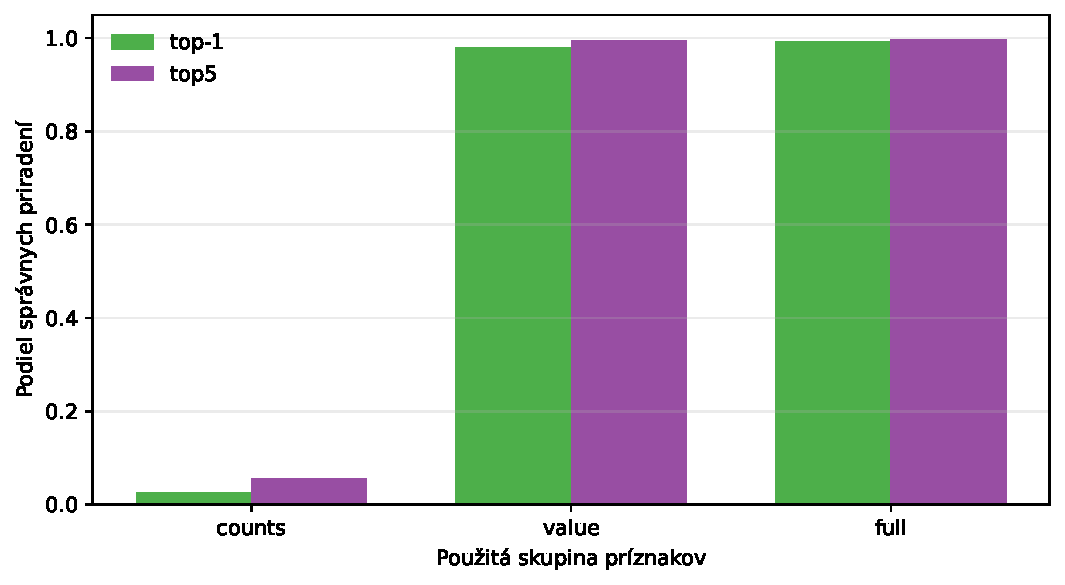
\includegraphics[width=0.82\textwidth]{img/generated/mapping_holdout_accuracy.pdf}
  \caption{Úspešnosť párovania na skrytej časti známych zhôd.
  Vlastné spracovanie.}
  \label{fig:mapping-accuracy}
\end{figure}

\subsection{Porovnanie klasifikačných modelov}

Každá výsledková tabuľka uvádza variant príznakov a grafu,
spôsob rozdelenia, počiatočnú hodnotu generátora, počty označených vrcholov v jednotlivých
častiach a počet použitých hrán. Bez týchto údajov by nebolo možné
rozlíšiť zlepšenie modelu od zmeny experimentálnej vzorky.

Pri náhodnom lese a GCN sa uvádza priemer a smerodajná odchýlka z
piatich počiatočných hodnôt. Logistická regresia je deterministická pri
pevnom vstupe. Rozdiel medzi časovým rozdelením a rozdelením odolným
voči úniku informácií sa
interpretuje spolu s počtom vyradených vrcholov. Pokles $F_1$ po
odstránení spoločných adries môže naznačovať, že pôvodný model využíval
opakované entity. Veľkosť jednotlivých mechanizmov úniku z neho určiť
nemožno.

Po odstránení adresného prekryvu ostalo 8~553 trénovacích, 5~808
validačných a 11~117 testovacích vrcholov. Vyradených bolo 2~743
vrcholov. Rekonštruovaný graf obsahuje 31~586 hrán medzi transakciami
s overeným mapovaním, kým pôvodný graf zvolených krokov obsahuje
31~653 hrán.

Obrázok~\ref{fig:split-retention} ukazuje, v ktorej časti sa počet
vrcholov zmenil. Tréning sa zmenšil iba o 13 nezmapovaných záznamov,
pretože pri prvej časti ešte neexistuje skoršia množina adries, s
ktorou by sa porovnávala. Väčší rozdiel vo validácii a teste vzniká
tým, že neskoršia transakcia sa odstráni, ak opakuje adresu prijatú v
skoršej časti. Graf zobrazuje technické čistenie aj zmenu populácie,
na ktorej sa model hodnotí.

\begin{figure}[htbp]
  \centering
  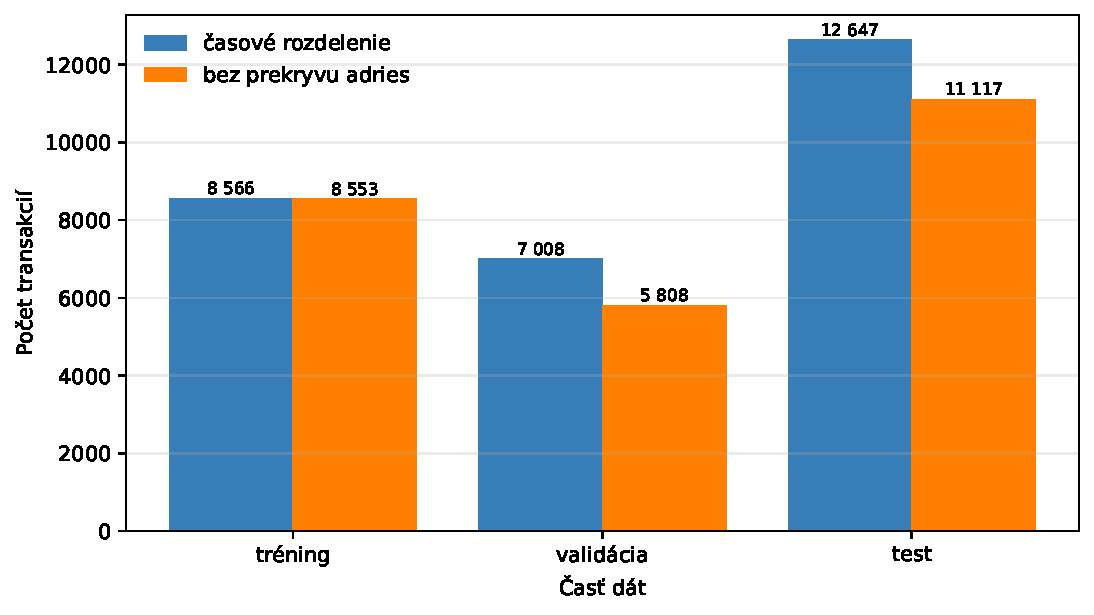
\includegraphics[width=0.82\textwidth]{img/generated/split_retention.pdf}
  \caption{Počet všetkých vrcholov pred odstránením a po odstránení
  pozorovateľného prekryvu adries. Vlastné spracovanie.}
  \label{fig:split-retention}
\end{figure}

Tabuľka~\ref{tab:model-results} uvádza priemernú hodnotu $F_1$ pre
ilicitnú triedu. Skratky A, B a C zodpovedajú variantom definovaným v
kapitole~\ref{sec:methodology}. Pri logistickej regresii sa smerodajná
odchýlka neuvádza, pretože pri pevnom vstupe prebehol jeden
deterministický výpočet.

\begin{table}[htbp]
  \centering
  \caption{Miera $F_1$ ilicitnej triedy; pri RF a GCN priemer
  $\pm$ smerodajná odchýlka z piatich počiatočných hodnôt. Vlastné spracovanie.}
  \label{tab:model-results}
  \begin{tabular}{llcc}
    \toprule
    Variant & Model & Časové rozdelenie & Bez prekryvu adries \\
    \midrule
    A & logistická regresia & 0,602 & 0,593 \\
    A & náhodný les & $0,820\pm0,013$ & $0,881\pm0,003$ \\
    A & GCN & $0,434\pm0,041$ & $0,437\pm0,019$ \\
    \midrule
    B & logistická regresia & 0,483 & 0,494 \\
    B & náhodný les & $0,734\pm0,081$ & $0,625\pm0,120$ \\
    B & GCN & $0,409\pm0,037$ & $0,392\pm0,021$ \\
    \midrule
    C & logistická regresia & 0,483 & 0,494 \\
    C & náhodný les & $0,734\pm0,081$ & $0,625\pm0,120$ \\
    C & GCN & $0,403\pm0,031$ & $0,392\pm0,021$ \\
    \bottomrule
  \end{tabular}
\end{table}

Najvyššiu hodnotu dosiahol náhodný les s pôvodnými príznakmi na
adresne oddelenom teste. Tento výsledok nemožno interpretovať ako
dôkaz, že únik informácií bol odstránený. Variant A stále obsahuje
adresné štatistiky vypočítané k budúcemu bloku 575~059 a oddelený test
má iné zloženie než pôvodný test. Porovnanie opisuje výsledok na
konkrétnej podmnožine; čistý kauzálny účinok jedného zásahu z neho
odvodiť nemožno.

Pri transparentných príznakoch klesol priemerný výsledok náhodného lesa
z 0,734 na 0,625 a variabilita medzi počiatočnými hodnotami vzrástla. Transparentný
vektor obsahuje 18 vlastností bez globálnej histórie adries.
Rozdiel oproti variantu A preto môže súvisieť súčasne s menším počtom
príznakov, odstránením budúcej informácie aj zmenou vzorky. Z tohto
experimentu nemožno tieto tri vplyvy číselne oddeliť.

Výsledky B a C sú pri logistickej regresii a náhodnom lese zhodné, čo
je očakávaná kontrola: tieto modely graf nepoužívajú. Pri časovom
rozdelení sa GCN po rekonštrukcii grafu zmenila z
$0,409\pm0,037$ na $0,403\pm0,031$. Pri adresne oddelenom rozdelení
majú oba grafy 25~619 povolených hrán, a preto poskytli zhodný súhrnný
výsledok $0,392\pm0,021$.

\begin{figure}[htbp]
  \centering
  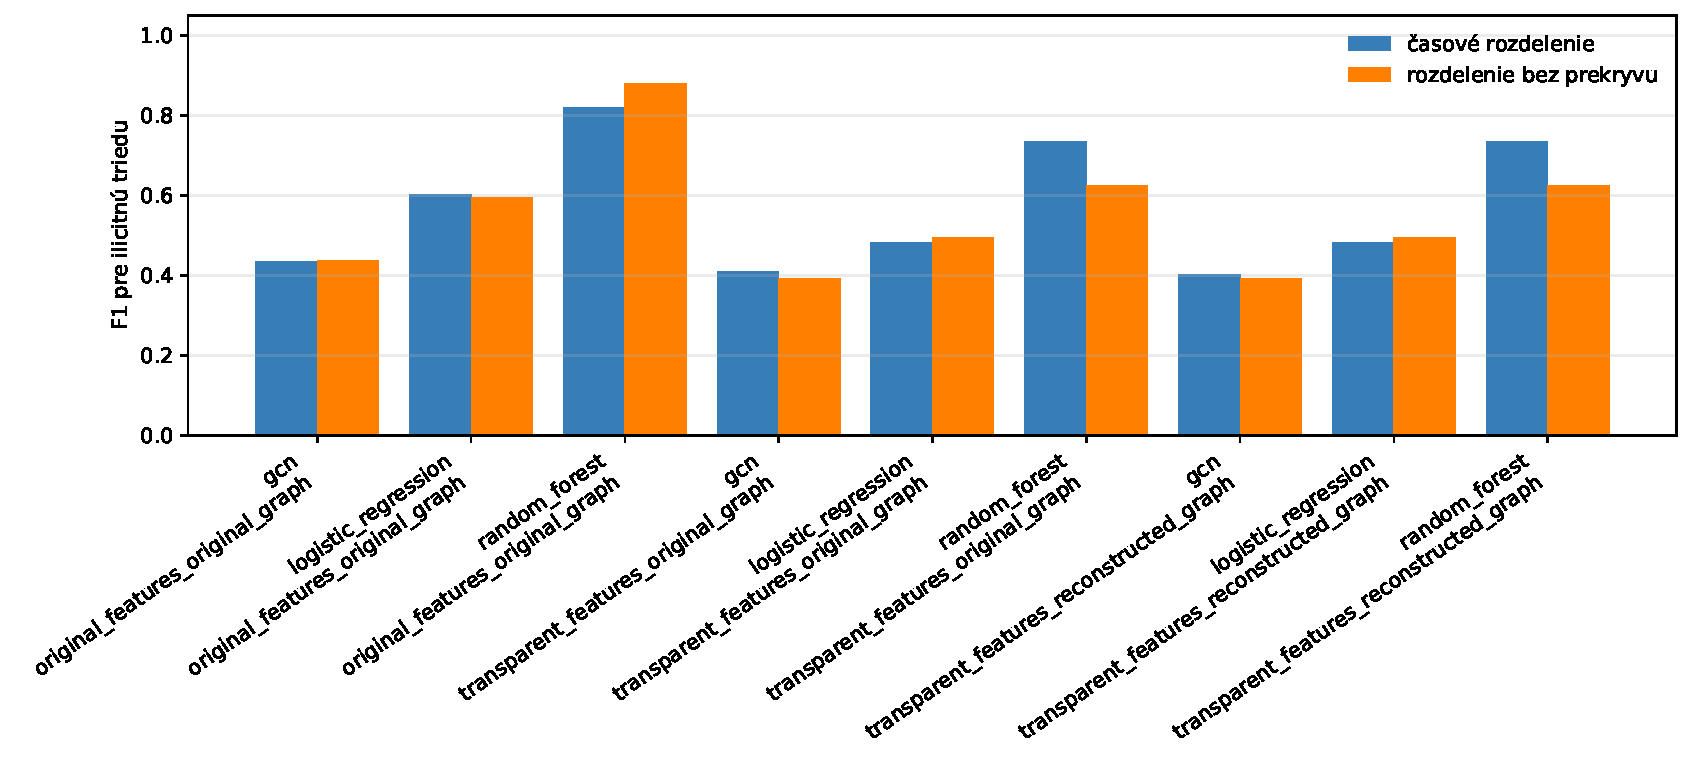
\includegraphics[width=\textwidth]{img/generated/model_f1_leakage_comparison.pdf}
  \caption{Porovnanie $F_1$ ilicitnej triedy pri dvoch spôsoboch
  rozdelenia. Vlastné spracovanie.}
  \label{fig:model-comparison}
\end{figure}

Miera $F_1$ spája precíznosť a úplnosť do jedného čísla. Smer zmeny
medzi väčším počtom upozornení a opatrnejšími predikciami ukazujú obe
zložky osobitne. Obrázok \ref{fig:metric-profile} preto rozkladá výsledok náhodného lesa s
transparentnými príznakmi na päť metrík. Každý stĺpec je priemer z
piatich behov. Precíznosť opisuje čistotu upozornení, úplnosť podiel
zachytených ilicitných označení a PR-AUC poradie skóre pri všetkých
prahoch. Graf tak zabraňuje interpretovať jednu hodnotu $F_1$ bez
informácie o type chýb.

\begin{figure}[htbp]
  \centering
  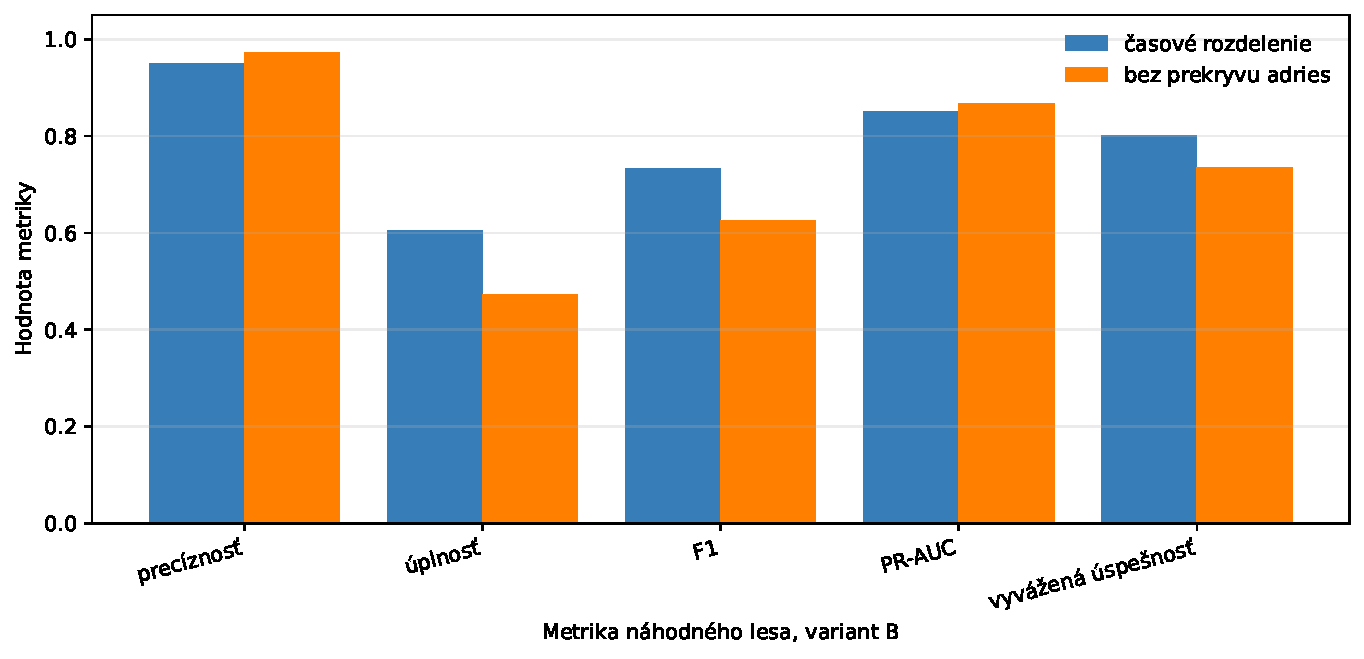
\includegraphics[width=0.92\textwidth]{img/generated/transparent_rf_metric_profile.pdf}
  \caption{Profil metrík náhodného lesa s transparentnými príznakmi,
  variant B. Stĺpce sú priemery z behov s počiatočnými hodnotami
  42--46. Vlastné
  spracovanie.}
  \label{fig:metric-profile}
\end{figure}

\begin{figure}[htbp]
  \centering
  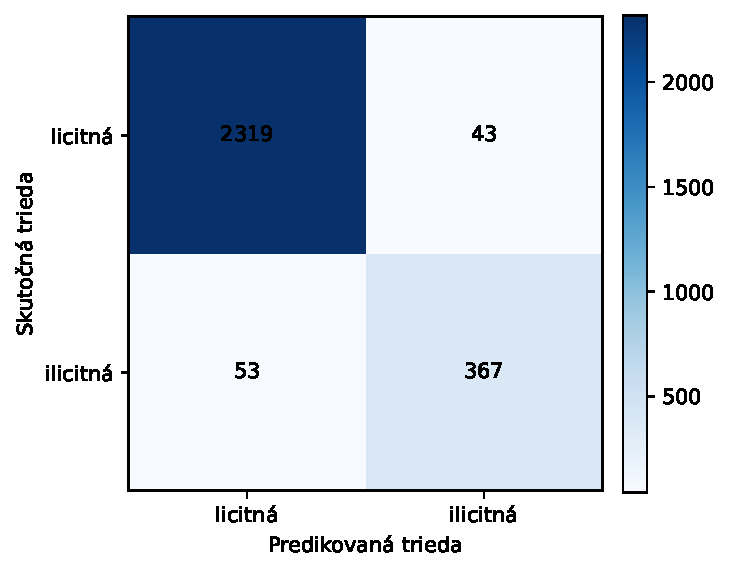
\includegraphics[width=0.55\textwidth]{img/generated/best_model_confusion_matrix.pdf}
  \caption{Matica zámen najlepšieho jednotlivého behu: náhodný les,
  variant A, rozdelenie bez prekryvu adries, počiatočná hodnota 45.
  Vlastné spracovanie.}
  \label{fig:confusion-matrix}
\end{figure}

\subsection{Hrozby pre platnosť}

Prvou hrozbou je správnosť verejného mapovania. Experiment so skrytou
kontrolnou časťou overuje schopnosť zopakovať známe zhody. Pôvod
každého riadka mapovania tým neoveruje. Druhou hrozbou je verejný Blockbook: server môže zmeniť
verziu alebo dočasne odmietnuť požiadavku. Manifest, vlastná hlavička
klienta a lokálna vyrovnávacia pamäť obmedzujú túto závislosť. Úplné
odstránenie by vyžadovalo vlastný zdroj blockchainových dát.

Treťou hrozbou je obmedzenie na šesť časových krokov. Výsledok nemožno
automaticky zovšeobecniť na celý Elliptic ani na súčasné bitcoinové
transakcie využívajúce novšie typy skriptov. Štvrtou hrozbou sú pôvodné
triedy. Zdrojová atribúcia entít nie je zverejnená, takže experiment
hodnotí reprodukciu tried Elliptic. Legalitu transakcií nezávisle
neurčuje.

Napokon, rozdelenie odolné voči úniku informácií odstraňuje transakcie
so spoločnými adresami. Dve odlišné adresy môžu naďalej patriť rovnakej
osobe. Postup kontroluje pozorovateľný prekryv adries; skutočných
vlastníkov nerozdeľuje.

